\documentclass[letterpaper, 12pt]{report}
\usepackage[top = 1.8cm, left = 3cm, right = 3cm ]{geometry}
\usepackage[pdftex]{graphicx}
\usepackage[francais]{babel}
\usepackage{amsmath}
\usepackage{amsthm}
\usepackage{url}
\usepackage{tikz}
\usepackage{float}
\usepackage{listings}
\usepackage[T1]{fontenc}
\usepackage[utf8]{inputenc}
\usepackage{epigraph}
\usepackage{fancyhdr}
\usepackage{gensymb}
\usepackage{rotating}
\usepackage[french,ruled,vlined]{algorithm2e}
\usepackage{longtable}
\usepackage{newfloat}
\usepackage{enumitem}
\usepackage{amsfonts}
\usepackage{textcomp}

\DeclareFloatingEnvironment[placement={!ht},name=List]{mylist}
\theoremstyle{definition}
\newtheorem{mydef}{Définition}
\newtheorem{myprop}{Propriété}
\newtheorem{mylemma}{Lemme}
\newtheorem{myexample}{Exemple}

\newcommand{\dom}{\mathbf{dom}}
\newcommand{\C}{\mathbb{C}}

\def\changemargin#1#2{\list{}{\rightmargin#2\leftmargin#1}\item[]}
\let\endchangemargin=\endlist 

\newcommand{\alinea}{
\hspace*{0.5cm}}

\renewcommand*\sfdefault{phv}
\renewcommand*\rmdefault{ppl}

\renewcommand\epigraphflush{flushright}
\renewcommand\epigraphsize{\normalsize}
\setlength\epigraphwidth{0.7\textwidth}

\definecolor{titlepagecolor}{RGB}{255,20,20}

\DeclareFixedFont{\titlefont}{T1}{phv}{\seriesdefault}{n}{0.375in}
  

\makeatletter
\setcounter{secnumdepth}{3} 
%\setcounter{tocdepth}{3} % makes the subsubsection appear in the table of content.
%\@addtoreset{section}{part}
%
%\renewcommand{\partname}{Partie}


% The following code is borrowed from: http://tex.stackexchange.com/a/86310/10898

\newcommand\titlepagedecoration{%
\begin{tikzpicture}[remember picture,overlay,shorten >= -10pt]

\coordinate (aux1) at ([yshift=-50pt]current page.north east);
\coordinate (aux2) at ([yshift=-380pt]current page.north east);
\coordinate (aux3) at ([xshift=-5cm]current page.north east);
\coordinate (aux4) at ([yshift=-130pt]current page.north east);
\coordinate (aux5) at ([yshift=-4cm]current page.north west);
\coordinate (aux6) at ([xshift=4cm]current page.north west);


\begin{scope}[titlepagecolor!40,line width=12pt,rounded corners=12pt]
\draw
  (aux1) -- coordinate (a)
  ++(225:5) --
  ++(-45:5.1) coordinate (b);
\draw[shorten <= -10pt]
  (aux3) --
  (a) --
  (aux1);
\draw[opacity=0.6,titlepagecolor,shorten <= -10pt]
  (b) --
  ++(225:2.2) --
  ++(-45:2.2);
\draw[opacity=0.5,titlepagecolor,shorten <= -15pt]
  (aux5) --
  (aux6);
\end{scope}
\draw[titlepagecolor,line width=8pt,rounded corners=8pt,shorten <= -10pt]
  (aux4) --
  ++(225:0.8) --
  ++(-45:0.8);

\begin{scope}[titlepagecolor!70,line width=6pt,rounded corners=8pt]
\end{scope}
\end{tikzpicture}%
}

\begin{document}
\begin{titlepage}

\noindent


\newgeometry{bottom = 2cm, top = 2.5cm}
\begin{center}

\includegraphics[scale=0.2]{umonslogo}\\
\vspace*{0.7cm}

\includegraphics[scale=0.32]{fs-logo}\\
\vspace*{2.5cm}
\titlefont Mémoire\\~\\{\LARGE  Data Repairing\\}~\\~\\{\large Réparation de contraintes} \par
\end{center}
\vspace*{3.5cm}
\hfill
\begin{minipage}{0.18\linewidth}
  \begin{flushright}
   \rule{0.5pt}{75pt}
  \end{flushright}
\end{minipage}
\begin{minipage}{0.8\linewidth}
\begin{flushleft}
\textsf{\textbf{Écrit par:}} Maxime Van Herzeele\\
\textsf{\textbf{Année académique:}} 2017-2018\\
\textsf{\textbf{Directeur de mémoire:}} Jef Wijsen\\
%\textsf{\textbf{Rapporteurs}} Pierre Hauweele \& Tom Mens\\
\textsf{\textbf{Section:}} MAB2 Sciences Informatiques
\end{flushleft}
\end{minipage}
\vspace*{\fill}
\begin{center}
Faculté des Sciences $\bullet$ University of Mons $\bullet$ Place du Parc 20 $\bullet$ B-7000 Mons
\end{center}
\titlepagedecoration
\end{titlepage}

\newgeometry{top = 3cm, left = 2.5cm, right = 2.5cm}

\pagestyle{fancy}
\lhead{Maxime Van Herzeele}
\rhead{MAB2 Computer Sciences}
\cfoot{\thepage}

\pagenumbering{roman} \setcounter{page}{1} 

%\section*{Remerciements} 
%\vspace*{0.8cm}
%\addcontentsline{toc}{section}{acknowledgement} 
%Todo : remerciement
%\newpage

\tableofcontents
\pagebreak
\listoffigures
\listoftables
\pagebreak

\chapter{Introduction}

\pagenumbering{arabic} \setcounter{page}{1} 

\alinea De nombreuses institutions et entreprises collectent, stockent et utilisent de grandes quantités d'informations. Le traitement de ces données permettent à ces entreprises d'effectuer des statistiques ou de fournir un service à l'un de leurs clients. Mais dans les bases de données, nous pouvons retrouver des données \emph{erronées}. Leur présence peut être due à une erreur lors de l'encodage ou lors de la collecte des informations(appareils imprécis, mauvaises méthodes de collecte, personne qui ment ou se trompe,...). Ces erreurs nuisent au traitement des données, biaisant les statistiques et perturbant les services qui en ont besoin. Afin d'éviter ce problème, les données devraient respecter des \emph{contraintes d'intégrité}. Une contrainte d'intégrité est une règle appliquée aux données. Si une donnée ne respecte pas au moins une de ses contraintes alors cette donnée doit être considérée comme erronée. \\

Malheureusement, il se peut que ces contraintes soient elles aussi erronées. A cause de ses erreurs sur les contraintes, celles-ci peuvent échouer dans la différenciation des données réellement erronées et des données correctes. Il se peut que certaines données soient identifiées comme étant des violations des contraintes (données erronées) malgré qu'elles ne le devraient pas. Il existe aussi des contraintes qui n'arrivent pas à détecter des violations. Les erreurs à la fois sur les données et sur les contraintes sont un problème pour quiconque souhaite utiliser la base de données\\

\begin{table}
\centering
\begin{tabular}{c|c c c c c}
 & Nome & Année & Salaire (\texteuro) & Grade & Bureau\\
 \hline
 $t_1$ & Dupont & 2012 & 23.000 & ouvrier & 1B18 \\
 $t_2$ & Dupont & 2013 & 24.000 & ouvrier & 1B14 \\
 $t_3$ & Dupont & 2014 & 38.000 & chef de service & 2B12 \\
 $t_4$ & Dupont & 2015 & 42.000 & chef de service & 2B18 \\
 $t_5$ & Dupont & 2016 & 37.000 & chef de service & 2B18 \\
 $t_6$ & Dupont & 2017 & 44.000 & chef de service & 2B18 \\
 $t_7$ & Dupont & 2018 & 28.000 & ouvrier & 1B14 \\
 $t_8$ & Ana & 2011 & 26.000 & ouvrier & 1B08 \\
 ... & & & & &\\
\end{tabular}

\caption{\label{exampleIntro}}
\end{table}


Par exemple, durant mon stage en entreprise, j'ai pu travailler sur un projet associé de près à une base de données ayant un problème de données erronées. Cela a eu un énorme impact sur une partie de mon projet. La réparation de ces données est prévue pour le courant de l'année 2018.\\

Le terme \emph{Data repairing} ou réparation de données signifie réparer les données mais aussi les contraintes d'intégrité. Il serait naïf de penser que l'on puisse supprimer chaque ligne qui possède au moins une donnée erronée. La perte d'information serait importante parce qu'une telle pratique demanderait d'effacer une ligne complète de la table et ce malgré qu'il n'y ait qu'une seule erreur dans la ligne. Par exemple, si nous avons une base de données des employés d'une entreprise et la contrainte "Le salaire d'un employé augmente chaque année". Cette contrainte n'est pas respectée à la table \ref{exampleIntro}. En effet, si nous prenons l'année 2016, nous voyons que monsieur Dupont gagne moins d'argent qu'en 2015 et 2014. Si nous supprimons l'année 2016, nous perdons l'information concernant le bureau que monsieur Dupont occupait.\\

En outre, les contraintes d'intégrité peuvent aussi être erronées ce qui veut dire que l'on pourrait supprimer une ligne ne contenant que des données correctes. Reprenons la contrainte "Le salaire d'un employé augmente chaque année". Cette contrainte n'est pas respecté à la table \ref{exampleIntro} car en 2017 Dupont gagnait 44.000 \texteuro et en 2018, il gagnait 28.000 \texteuro de salaire annuel. Nous avons l'une des deux lignes de la table qui contient une donnée erronée. Mais c'est sans compter sur le fait que monsieur Dupont a perdu son grade de chef. Du coup la contrainte est peut être erronée et la contrainte "Le salaire d'un employé augmente chaque année à condition de garder son grade" est correcte. Dans ce cas ci, l'erreur ne vient pas des données mais de la contrainte. Pour cette raison, nous avons besoin de techniques afin de réparer à la fois les données et les contraintes, ce sans perdre trop d'informations tout en évitant d'échouer dans la détection d'erreurs dans les données.\\

Dans cette thèse de mémoire, nous allons analyser le \emph{modèle de réparation $\theta$-tolérant} comme il a été introduit dans un article scientifique\cite{main}. Nous allons faire varier nos contraintes et chacune de nos variations aura un coût que nous devrons déterminer. Le coût de toutes ces variations ne devra pas excéder $\theta$. Le nouvel ensemble de contraintes sera utilisé pour la réparation des données.\\

Dans un premier temps, nous allons introduire le concept de \emph{denial constraint}, une forme de contraintes d'intégrité qui va nous aider à définir et comprendre le concept du modèle de réparation $\theta$-tolérant. Nous allons également introduire quelques bases de données que nous utiliserons pour illustrer les différentes notions que nous allons aborder. Ensuite, nous allons présenter des techniques pour faire varier nos denial constraint en respectant le modèle de réparation $\theta$-tolérant. Puis, puisque nous resterons critique par rapport au papier scientifique de référence, nous expliquerons en quoi notre démarche est différente et pourquoi nous avons choisi de modifier certaines approches et certains concepts. Enfin, nous terminerons avec une implémentation du modèle $\theta$-tolérant et analyserons ses performances avec quelques exemples.


\chapter{Les contraintes d'intégrité}

\alinea Dans ce chapitre, nous allons rappeler quelques notions bien connues mais nous allons également introduire de nouveaux concepts. Dans un premier temps, nous allons présenter quelques bases de données que nous utiliserons en tant qu'exemple pour expliquer et illustrer de nombreuses propriétés et définitions. Ces bases de données suivent le modèle relationnel qui a été introduit par E.F. Codd \cite{misc1}. Ensuite nous allons travailler sur les contraintes d'intégrité et nous allons introduire un nouveau type de contraintes appelées \emph{denial constraint}. Nous allons expliquer plusieurs caractéristiques et propriétés de ces contraintes et expliquer pourquoi nous n'utilisons pas une forme plus conventionnelle de contrainte, comme par exemple les dépendances fonctionnelles.

\section{Base de données}

\alinea Dans cette section, nous allons présenter des bases de données que nous allons utiliser comme exemple dans cette thèse de mémoire. Nous utiliserons ces bases de données pour illustrer le modèle de réparation de données $\theta$-tolérant ainsi que d'autres notions que nous définirons.\\

La première base de données est tirée de l'article principal utilisé dans la bibliographie de cette thèse \cite{main}. Elle représente une table de personnes comprenant le nom de ces personnes, leur date de naissance, leurs numéros de téléphone, leurs revenus, le montant de taxe que ces personnes paient ainsi que l'année à laquelle toutes ces données ont été encodées.

\begin{table}[H]
	\centering
	\begin{tabular}{|c|c c c c c c|}
	\hline
	    & Nom & Anniversaire & NumTel & Année & Revenu & Taxe\\
	\hline
	 t1 & Ayres & 8-8-1984 & 322-573 & 2007 & 21k & 0\\
	 t2 & Ayres & 5-1-1960 & ***-389 & 2007 & 22k & 0 \\
	 t3 & Ayres & 5-1-1960 & 564-389 & 2007 & 22k & 0 \\
	 t4 & Stanley & 13-8-1987 & 868-701 & 2007 & 23k & 3k\\
	 t5 & Stanley & 31-7-1983 & ***-198 & 2007 & 24k & 0\\
	 t6 & Stanley & 31-7-1983 & 930-198 & 2008 & 24k & 0\\
	 t7 & Dustin & 2-12-1985 & 179-924 & 2008 & 25k & 0 \\
	 t8 & Dustin & 5-9-1980 & ***-870 & 2008 & 100k & 21k \\
	 t9 & Dustin & 5-9-1980 & 824-870 & 2009 & 100k & 21k \\
	 t10 & Dustin & 9-4-1984 & 387-215 & 2009 & 150k & 40k \\
	 \hline
	\end{tabular}
	\caption{\label{tableMain} Base de données de l'article principal \cite{main}}.
\end{table}

La seconde base de données que nous allons utiliser est inspirée d'une expérience personnelle. Lors d'un stage en entreprise, j'ai pu travailler sur un projet lié à une base de donnée contenant des données erronées. Ces données ne pouvant pas être utilisées en dehors de l'entreprise, nous utiliserons une base de données reprenant l'idée générale. C'est une table appelée "Personne" contenant différentes informations basiques sur des personnes en Belgique \footnote{Les données sont fictives} . 

\begin{itemize}
\item \textbf{NISS:} Le numéro national de la personne. Un numéro national est unique. En règle général, un NISS est formé de la manière suivante: \cite{bcss}
	\begin{itemize}
	\item Il commence avec la date de naissance de la personne dans un format YY-MM-DD. Des exceptions existent pour les étrangers (c'est à dire des personne n'ayant pas la nationalité belge) mais nous n'allons pas considérer ces cas. En effet ces cas peuvent être difficiles à comprendre et ne sont aucunement intéressants pour la suite.
	\item Le nombre composé du septième, huitième et neuvième chiffres est pair pour les hommes et impair pour les femmes
	\item Le nombre composé des deux derniers chiffres est le resulat de $n \mod 97$ avec n le nombre formé des 9 premiers chiffres
	\end{itemize}
\item \textbf{Nom:} Nom de famille de la personne.
\item \textbf{Prénom:} Prénom de la personne.
\item \textbf{Nai\_Date:} Date de naissance de la personne dans le format DD-MM-YYYY.
\item \textbf{Dec\_Date:} Date de décès de la personne dans le format DD-MM-YYYY.
\item \textbf{Etat\_Civil:} État civil courant de la personne, celui ci doit être parmi les suivants : (célibataire, marié, divorcé, décédé, veuf)
\item \textbf{Ville} : La ville où la personne vit.
\item \textbf{Code\_Post} : Le code postal de la ville.
\item \textbf{Salaire} : Le salaire perçu par la personne en une année.
\item \textbf{Taxe} : Le montant de taxe payé par la personne en une année.
\item \textbf{Enfant} : Le nombre d'enfants que la personne a à charge.
\end{itemize}

\begin{table}[H]
 \footnotesize	
	\centering
	\hspace*{-2cm}\begin{tabular}{|c|c c c c c c c c c c c|}
	\hline
	    & Niss & Nom & Prénom & Nai\_Date & Dec\_Date & Etat\_Civil & Ville & Code\_Post & Salaire & Taxe & Enfant\\
	\hline
	 t1 & 14050250845 & Dupont & Jean & 14-05-1902 & 18-05-1962 & décédé & Ath & 7822 & 25k & 4k & 2\\
	 t2 & 08042910402 & Brel & Jacques & 08-04-1929 & 09-10-1978 & décédé & Schaerbeek & 1030 & 100k & 8k & 1\\
	 t3 & 45060710204 & Merckx & Eddy & 07-06-1945 & null & décédé & Schaerbeek & 1030 & 125k & 9k & 2\\
	\hline
	 
	 \hline
	\end{tabular}
	\caption{\label{tablePerson} La table Personne}.
\end{table}


\newpage

\section{Contraintes sur les bases de données}

\alinea Les bases de données devraient n'accepter que des valeurs qui respectent certaines normes et règles. Ce serait un problème si on pouvait ajouter n'importe quelle valeur à chaque colonne d'une base de données. Pour éviter ce problème, nous avons recours à des règles sur les bases de données. Ces règles sont appelées \emph{contraintes d'intégrité} et fonctionnent de la manière suivante: Si une relation i.e un ensemble de tuples respecte toutes les conditions de ces contraintes alors les données sont acceptables. Si la relation ne respecte pas toutes les conditions alors au moins un tuple de la relation contient au moins  une valeur erronée. \\

Le modèle relationnel des bases de données introduit la notion de \emph{dépendance fonctionnelle}:

\begin{mydef}
Une \textbf{dépendance fonctionnelle (DF)} est une expression $X \rightarrow Y$ avec $X,Y \subseteq
sort(R)$ et où $sort(R) = \{ A_1,A_2,...,A_n\}$ signifient que pour chaque ensemble de tuples où les attributs de X correspondent, on a les attributs de Y qui correspondent aussi.
\end{mydef} 

En d'autres mots, la contrainte $X \rightarrow Y$ signifie que pour une valeur spécifique de X, il n'y a au plus une valeur possible pour Y. Si la DF est respectée sur la relation R, nous pouvons dire que R satisfait la DF. Prenons quelques exemple sur la table \ref{tablePerson}:

\begin{enumerate}
\item \emph{Un NISS identifie une personne}: En d'autre mot, pour une valeur spécifique du NISS, il n'y a qu'une seule valeur possible pour tout les autres attributs de la table. Cela peut se décrire par la DF suivante:
$ NISS \rightarrow Nom, Prenom, Nai\_Date, Dec\_Date, Etat\_Civil, Ville,$ $Code\_Post, Salaire, Taxe, Enfant$
\item \emph{Deux personnes avec le même code postal vivent dans la même ville.} : Pour une valeur spécifique de $Code\_Post$ dans notre table il n'y a qu'une valeur possible de $Ville$. Par exemple si la valeur de $Code\_Post$ d'une personne est '7822', la seule valeur possible pour l'attribut $Ville$ est 'Ath'. La dépendance fonctionnelle dans ce cas est $Code\_Post \rightarrow Ville$.
%\item \emph{If someone died the march 18$^{th}$ 1962 , his civil status should be equal to decease.} : In this case we need a conditional functional dependency(CFD) which is typically a functional dependency with equality operator on some columns. A functional dependency should work for all records on the table, CFD can hold some conditions on collumns. $[Decease\_date = $'18-05-1962'$] \rightarrow [civil\_status = decease]$
\end{enumerate}

\begin{mydef}
Si pour chaque paire de tuples de la relation $R$, la DF $\tau$ est respectée, nous disons que la relation $R$ \emph{satisfait $\tau$}. Cela ce note $R \models \tau$.
\end{mydef}

Évidement, certaines bases de données ne contiennent pas qu'une seule contrainte mais plusieurs. Il est important qu'elles soient toutes respectées. Ce qui nous conduit à la définition suivante:
  
\begin{mydef}
Soit un ensemble $\Sigma$ de DF sur la relation $R$. On dit que la relation $R$ satisfait $\Sigma$ noté $R \models \Sigma$ si pour chaque DF $ \tau \in \Sigma$, on a $R \models \tau$
\end{mydef}

Malheureusement, les dépendances fonctionnelles sont limitées en terme de puissance. En effet, il existe de nombreuses contraintes que nous ne pouvons pas exprimer avec une DF. Par exemple, si nous souhaitons exprimer le fait que \emph{`La date de naissance d'une personne doit être antérieure à sa data de décès'}, nous avons besoin de comparer la $Nai\_Date$ et la $Dec\_Date$ de la personne et de s'assurer que la date de décès ne soit antérieure à la date de naissance. Les dépendances fonctionnelles ne permettent pas d'utiliser des opérateurs de comparaison, il est donc nécessaire d'exprimer les contraintes d'une autre façon. Pour ce faire, nous allons introduire un nouveau type de contrainte qui répondra bien à nos besoins: les \emph{denial constraints}.

\section{Les Denials constraints}

Dans cette section, nous allons définir ce qu'est une denial constraint. Nous allons aussi expliquer son utilisation dans les bases de données et nous allons également lister et expliquer plusieurs propriétés que peuvent avoir ces contraintes. Commençons d'abord par définir la denial constraint

\begin{mydef}
Considérons un ensemble $S$ fini d'\emph{attribut}. Une \emph{denial constraint (DC)} sur l'ensemble $S$ est une fonction partielle de $S$ vers l'ensemble des parties(aussi appelé ensemble puissance) de $\{ <,=,> \}$ noté $OP$. Nous utiliserons la lettre grecque $\varphi$ pour représenter une DC. Chaque parties de $OP$ se nomme \emph{opérateur}.
\end{mydef}

\begin{mydef}
 Soit $(\dom,\leq)$ un domaine totalement ordonné contenant au moins deux éléments distincts. Un \emph{tuple sur $S$} est une fonction totale de S à $\dom$. Une \emph{relation sur S} est un ensemble fini de tuples sur $S$. 
\end{mydef}

Par définition l'ensemble puissance d'un ensemble $S$ noté $\mathcal{P}(S)$ est l'ensemble de tous les sous-ensembles de $S$. Cela inclut l'ensemble $S$ lui même mais aussi l'ensemble vide $\emptyset$. Par exemple $OP$ (l'ensemble des parties de $\{ <, =, > \}$) est $\mathcal{P}(OP)$ = $\{ \emptyset, \{<\} , \{=\}, \{>\}, \{<,=\}, \{=,>\}, \{<,>\}, \{<,=,>\} \}$. Nous utiliserons la lettre grecque $\phi$ ou $\theta$ pour représenter un opérateur. Il existe différentes abréviations pour les éléments de $OP$, ceux-ci étant répertoriés dans la table \ref{operatorTable}. Nous avons eu besoin d'introduire 2 nouveaux opérateur $\top$ et $\bot$, chacun étant l'abréviation pour l'ensemble $\{<,=,>\}$ et $\emptyset$ respectivement. Nous les définissons comme tel: 
\begin{mydef}$ \forall a,b \in \mathbf{dom}$,nous avons $a \bot b$ est toujours faux et $a \top b$ est toujours vrai. 
\end{mydef}

\begin{table}
	\begin{center}
	\begin{tabular}{|c|c|c|c|}\hline
	$\theta$ & Abréviation & $\bar{\theta}$ & $\hat{\theta}$ \\\hline\hline
	$\emptyset$ & $\bot$ & $\top$ & $\bot$ \\\hline
	$\{<\}$     & $<$ & $\geq$ & $>$ \\\hline
	$\{=\}$     & $=$ & $\neq$ & $=$ \\\hline
	$\{>\}$     & $>$ & $\leq$ & $<$ \\\hline 
	$\{<,=\}$   & $\leq$ & $>$ & $\geq$ \\\hline 
	$\{<,>\}$   & $\neq$ & $=$ & $\neq$ \\\hline
	$\{>,=\}$   & $\geq$ & $<$& $\leq$ \\\hline 
	$\{<,=,>\}$ & $\top$ & $\bot$ & $\top$ \\\hline
	\end{tabular}
	\end{center}
	\caption{Element de OP, l'ensemble des parties de $\{ <,=,>\}$ \label{operatorTable}}
\end{table}

Expliquons maintenant la sémantique qui se cache derrière la denial constraint.

\begin{mydef}
\label{defSatisf}
On dit qu'une relation $I$ sur $S$ \emph{satisfait} la DC $\varphi$, noté $I \models \varphi$ si il \textbf{n'existe pas} deux tuples $s,t \in I$ tel que pour chaque attribut $A$ dans le domaine de $\varphi$, nous avons $s(A)\theta t(A)$ avec $\theta =  \varphi(A)$ 
\end{mydef}

Notons que les tuples $s$ et $t$ ne doivent pas forcément être distinct.  La relation $I$ peut être vide. Une relation vide satisfait toutes les DCs.

\begin{myexample}
Prenons un exemple sur la table \ref{tableMain}, nous avons $S=\{Nom, Anniversaire, NumTel,$ $Annee, Revenu, Taxe \}$ Une DC pour S est $\varphi =\{(Nom,=),(Anniversaire,=),(NumTel,\neq),(Annee,\top),(Revenu,\top) ,(Taxe,\top) \}$. Celle-ci est satisfaite par la relation $I$ si il n'existe pas deux tuples $s,t\in I$ tel que $s(Nom) = t(Nom) \wedge s(Anniversaire) = t(Anniversaire) \wedge s(NumTel) \neq t(NumTel) \wedge s(Annee) \top y(Annee) \wedge s(Revenu) \top t(Revenu) \wedge s(Taxe) \top t(Taxe)$.
\end{myexample}

Lorsqu'une relation $I$ sur $S$ ne satisfait pas une DC $\varphi$, on dit que $I$ \emph{viole} $\varphi$ que l'on note $I \not\models \varphi$. Chaque élément de $\varphi$ est appelé un prédicat. Pour chaque prédicat $(A,\theta)$, on appelle $A$ l'attribut du prédicat, et $\theta$ l'opérateur du prédicat.  Soit $I$ une relation sur $S$ et $\varphi$ une DC. Dès lors on peut dire que $I \models \varphi$ si pour tout $s,t \in I$ au moins un des prédicats est faux pour $\{s,t\}$ i.e pour au moins un prédicat $(A,\theta_A)$ on a $s.A \theta_A t.A$ qui est faux. Si un prédicat $P$ a pour opérateur $\top$ alors $P$ sera toujours vrai pour tout $t,s \in I$. Dès lors à l'avenir, nous ne noterons plus les prédicats ayant $\top$ pour opérateur par facilité syntaxique. L'exemple précédent s'écrira désormais $\varphi =\{(Nom,=),(Anniversaire,=,?(NumTel,\neq)\}$. Si un prédicat a pour opérateur $\bot$, il sera toujours faux. Dès lors $I \models \varphi$. Notons que la relation vide est la seule relation qui satisfait la DC $\varphi = \{(A_1,\top),(A_2,\top),...(A_n,\top)\} \equiv \{ \}$.\\

 Si nous prenons l'instance $I$ comme étant la table \ref{tableMain}, nous avons $I \not\models \varphi$. En effet prenons $s=t_2$ et $t=t_3$ nous avons bien $t_2(Nom) = t_3(Nom) \wedge t_2(Anniversaire) = t_2(Anniversaire) \wedge y_2(NumTel) \neq t_3(NumTel)$. On dit que $\{ t_2,t_3 \}$ \emph{viole} la contrainte $\varphi$\\ 

Pour chaque opérateur dans $OP$ nous pouvons définir son inverseet sa réciproque. Les valeurs de l'inverse et de la réciproque de chaque élément de $OP$ se trouve également à la table \ref{operatorTable}.
\begin{mydef}
Soit $\phi$ un élément de $OP$

L'inverse de $\phi$ noté $\overline{\phi}$ est égal à $\{<,=,>\}\setminus \phi$

La réciproque de $\phi$ noté $\hat{\phi}$ s'obtient en inter-changeant < et > dans $\phi$

\end{mydef}

Une DC peut être \emph{sur-simplifiée} ce qui veut dire qu'une donnée correcte peut être considérée comme une violation. Prenons un exemple sur la table \ref{tableMain} avec la denial constraint suivante:

$$\varphi_2 = (Nom,=)(NumTel,\neq) $$

Cette contrainte veut dire que si une personne possède le même nom qu'une autre, alors elle ne peut pas avoir un numéro de téléphone différent. Ceci est bien sur incorrect. En effet, deux personnes différentes ne peuvent avoir le même numero de téléphone. Dans notre relation, le nom seul ne suffit pas à identifier si deux personne sont identiques. Prenons par exemples $t_1$ et $t_2$, ils ne satisfont pas $\varphi_2$. Si l'on regarde de plus près, on peut facilement comprendre qu'il s'agit de deux personnes différentes. Ces deux personnes n'ont pas le même age i.e elles ont une date d'$Anniversaire$ différent. Si nous souhaitons améliorer la précision de la contrainte et éviter que $\langle t_1,t_2\rangle$ soit considéré comme une violation, nous avons besoin de regarder l'attribut $Anniversaire$. Une meilleure DC serait:

$$\varphi_2' = (Nom,=),(Anniversaire,=),(NumTel,\neq) $$

Une DC peut être également \emph{sur-raffiné} ce qui entraine qu'une donnée erronée peut être considérée comme correcte par la DC. Prenons un exemple sur la table \ref{tableMain} avec la denial constraint suivante:

$$\varphi_2' = (Nom,=),(Anniversaire,=),(NumTel,\neq),(Annee,=) $$

Dans ce cas, l'information $Annee$ n'est pas utile pour distinguer deux personnes différentes. Dans la table, l'attribut année correspond à l'année où les autres attributs ont été encodés. Une même personne peut être encodée deux fois à deux années différentes. Avec cette DC, on ne reconnait pas $\{ t_5,t_8 \}$ comme étant une violation.

%\newpage
%----------\\
%Une DC est un fonction partielle de l'ensemble $S$ des attributs vers $OP$. Reprenons nos exemples sur les DF et essayons de les exprimer en terme de DC. Pour notre table \ref{tablePerson}, nous avons l'ensemble $S=\{NISS, Nom, Prénom, Nai\_Date, Dec\_Date, Etat\_Civil, Ville, Code\_Post, Salaire, Taxe, Enfant \}$.
%\begin{itemize}
%\item \emph{Un NISS identifie une personne.}: $\{ (NISS,=), (Nom,\neq) (Prénom,\neq), (Nai\_Date,\neq), (Dec\_Date,\neq), (Etat\_Civil,\neq), (Ville,\neq), (Code\_Post,\neq), (Salaire,\neq), (Taxe,\neq), (Enfant,\neq) \}$
%\item \emph{Deux personnes avec le même code postal vivent dans la même ville.}: $\{ (NISS,\top), (Nom,\top) (Prénom,\top), (Nai\_Date,\top), (Dec\_Date,\top), (Etat\_Civil,\top), (Ville,\neq), (Code\_Post,=), (Salaire,\top), (Taxe,\top), (Enfant,\top) \}$ . On peut également l'écrire $\{ (Ville,\neq), (Code\_Post,=) \}$
%\end{itemize}
%---------

\subsection{Quelques définitions et propriétés}

Dans cette sous-section, nous allons définir quelques notions et propriétés sur les DC qui nous serviront dans les chapitres qui suivront.
\subsubsection{Satisfiabilité}

\begin{mydef}
Soit $\varphi$ DC sur $S$. On dit que $\varphi$ est \emph{satisfiable} si elle peut être satisfaite par une relation non vide sur $S$, i.e si $\exists I$ sur $S$ avec $I$ non vide tel que $I \models \varphi$, alors $\varphi$ est \emph{satisfiable}.

Si $\varphi$ n'est pas satisfiable, nous dirons qu'il est \emph{insatisfiable} 
\end{mydef}

Il est intéressant de savoir à l'avance si une une denial constraint est satisfiable ou pas. Le lemme suivant nous permet de détecter les DC qui ne sont pas satisfiables.

\begin{mylemma}\label{satisLemma}
	Soit $\varphi$ une denial constraint sur $S$, alors $\varphi$ est satisfiable si et seulement si il existe un prédicat $P_i \in pred (\varphi)$ de la forme $(A_i,\theta_i)$ tel que $\theta_i$ ne contient pas $=$, i.e $\theta_i \not\in \{ \{=\},\{<,=\},\{=,>\},\{<,=,>\},\} $ 
\end{mylemma}
\begin{proof}~\\
\alinea \framebox{$\implies$} Supposons que pour tout $P \in pred(\varphi)$, $\theta$ contient $=$. Alors pour chaque tuple $s$ sur $S$, pour chaque $P_i \in pred(\varphi)$ on a $s(A_i) \theta_i s(A_i)$. Il s'ensuit que toute relation non vide ne satisfait pas $\varphi$

\framebox{$\impliedby$} Supposons $B \in S$ tel que $B$ ne contient pas $=$. Alors pour chaque tuple $s$ sur $S$, nous avons que $s(B)\ \theta s(B)$ avec $\theta=\varphi(B)$ faux. Il s'ensuit que n'importe quelle relation avec exactement un tuple satisfait $\varphi$.

\end{proof}


\subsubsection{Implication logique}

\begin{mydef}
Soit $\varphi_1,\varphi_2$ deux DC sur $S$. On dit que $\varphi_1$ \emph{implique (logiquement)} $\varphi_2$, que l'on note $\varphi_1 \models\varphi_2$, si pour chaque relation $I$ sur $S$, si $I \models \varphi_2$ alors on a $I \models \varphi_1$. On dira aussi que $\varphi_2$ est \emph{plus faible} que $\varphi_1$ ou bien que $\varphi_1$ est \emph{plus fort} que $\varphi_2$
\end{mydef}

\begin{myexample}
%Soit $S=\{Nom,Anniversaire,NumTel,Année,Revenu,Taxe \}$ et deux DC $\varphi_1 = \{ (Salaire,\leq)(Taxe,\geq) \}$ et $\varphi_2 = \{ (Salaire,<)(Taxe,>) \}$$ Prenons une relation I qui satisfait $\varphi_1$
Soit $S=\{A,B\}$.
Soit $\varphi_1=\{(A,\leq),(B,\neq)\}$ et $\varphi_2=\{(A,<),(B,>)\}$.
Alors $\varphi_1$ implique $\varphi_2$.
En effet, soit $I$ une relation qui satisfait $\varphi_1$.
Alors pour tout tuples $s,t\in I$, on a $s(A)>t(A)$ ou bien $s(B)=t(B)$ (ou éventuellement les deux en même temps).
Il s'ensuit que pour tout tuples $s,t\in I$, on a $s(A)\geq t(A)$ ou bien $s(B)\leq t(B)$ (ou les deux en même temps).
Dès lors, $I$ ne contient pas deux tuples $s,t$ tel que  $s(A)<t(A)$ et $s(B)>t(B)$.
On a donc $I$ qui satisfait $\varphi_2$.
D'un autre côté, $\varphi_2$ n'implique pas $\varphi_1$.
En effet, considérons la relation $I$ suivante.
$$
\begin{array}{c|cc}
I & A & B\\\cline{2-3}
  & 1 & 2\\
  & 1 & 3
\end{array}  
$$
Dès lors, nous avons $I\models\varphi_2$, mais $I\not\models\varphi_1$.
\end{myexample}

\begin{mylemma}\label{lem:characterization}
Soit $\varphi_1$ et $\varphi_2$ deux denial constraints sur $S$.
Si $\varphi_2(A)\subseteq\varphi_1(A)$ $\forall A\in S$, alors $\varphi_1\models\varphi_2$.
\end{mylemma}
\begin{proof}
Supposons que $\varphi_2(A)\subseteq\varphi_1(A)$ pour tout $A\in S$.
Soit $I$ une relation sur $S$ tel que $I\models\varphi_1$.
Nous avons besoin de démontrer que $I\models\varphi_2$.
Soit $s,t\in I$.
Puisque $I\models\varphi_1$, nous pouvons supposer l'existence d'un $A\in S$ tel que $s(A)\ \theta\ t(A)$ est faux, avec $\theta=\varphi(A)$. 
Puisque $\varphi_2(A)\subseteq\varphi_1(A)$,
alors nous aurons $s(A)\ \theta'\ t(A)$ est faux, avec $\theta'=\varphi_2(A)$.
\end{proof}

\begin{myexample}
 $\{(A,=)\}\models\{(A,\leq)\}$. car $\{=\} \subseteq \{<,=\} \equiv \leq$
\end{myexample}

\subsubsection{Trivialité}

Une DC peut être inutile et toujours vraie. De telles DC ne devraient pas être présentes dans la base de données puisqu'elles ne détecteront jamais aucune violation. Dans ce cas, on dira que la DC est \emph{triviale}. 
\begin{mydef}
	Une DC $\varphi$ est dite \emph{triviale} si $\forall I$ sur S, on a $I \models \varphi$
\end{mydef}

\begin{mylemma} \label{trivialLemma}
Soit $\varphi$ une DC sur $S$. alors $\varphi$ est triviale si et seulement si $\theta = \bot$ pour un prédicat de la forme $P=(A,\theta) \in pred(\varphi)$.
\end{mylemma}
\begin{proof}
~\\
\alinea \framebox{$\implies$}
Supposons que pour chaque prédicat $P=(A,\theta) \in pred(\varphi)$ avec $\theta \neq \bot$. Soit $s,t$ deux tuples tel que pour chaque $P=(B,\theta)$, nous avons $s(B)\ \theta\ t(B)$ vrai.
Puisque $\theta \neq \bot$ et que $\dom$ contient au moins deux éléments, $s,t$ peuvent être construit. Dès lors $\{s,t\}$ ne satisfont pas $\varphi$ puisque $\varphi$ n'est pas triviale.

\framebox{$\impliedby$}
Supposons qu'il existe un prédicat $P=(A,\theta) \in pred (\varphi)$ tel que $\theta = \bot$.
Puisque $s(A) \bot t(A)$ est faux pour tout tuples $s,t$ sur $S$, aucune relation ne peut contenir deux tuples $s,t$ tel que $s(A) \bot t(A)$ est vrai.
\end{proof}

%TODO : trouver un exemple

\subsubsection{Augmentation}

Dans les chapitres suivants, nous verrons comment nous pouvons améliorer les DCs afin qu'elles puissent détecter les données erronées de manière correcte. Pour ce faire nous aurons besoin de modifier des prédicats et donc de changer les opérateurs de ceux ci. Mais modifier un opérateur $\top$ est inutile par la propriété suivante:

\begin{myprop}
%	If $\varphi = \neg (P_1 \wedge P_2 \wedge ... \wedge P_n)$ is a valid DC, then $\varphi ' = \neg(P_1 \wedge P_2 \wedge ... \wedge P_n \wedge Q)$ is also a valide DC
	Soit une DC $\varphi$ sur S et une relation $I$ tel que $I \models \varphi$. Si il existe un prédicat $P_i = (A_i,\theta_i) \in pred(\varphi)$ tel que $\theta_i = \top$ alors pour la DC $\varphi'$ tel que $pred( \varphi' ) = pred( \varphi ) \textbackslash P_i$ avec $P_i' =(A_i,\theta_i)$ et $\theta_i \neq \top$, on a $I \models \varphi'$
\end{myprop}



Cette propriété est triviale. Souvenons nous que $\varphi$ est un DC tel que $I \models \varphi$ donc $\forall t \in I$ on a $\varphi$ vrai. Imaginons que $\varphi$ contienne le prédicat de la forme $(A,\top)$ Prenons $\varphi'$ une DC qui est la variante de $\varphi$ tel que $pred(\varphi) =  pred(\varphi')$ à l'exception du prédicat $(A,\top)$ qui devient $(A,\theta)$ avec $ \theta \neq \top$. Puisque $\varphi$ était satisfaite par $I$, il y avait déjà un autre prédicat de $\varphi$ qui était faut $\forall t \in I$. Donc $\varphi'$ est satisfaite pour qu'importe la valeur de $(A,\theta)$.

\subsubsection{Transitivity}
%In \cite{DCs} they defined the transitivity of DCs as:
%
%\begin{myprop}
%	If $\varphi = \neg (P_1 \wedge P_2 \wedge ... \wedge P_n \wedge Q_1)$ and $\varphi ' = \neg (R_1 \wedge R_2 \wedge ... \wedge R_n \wedge Q_2)$ are both valid DCs and $Q_2 \in Imp(\overline{Q_1})$, \\ then $ \varphi '' = \neg(P_1 \wedge ... \wedge P_n \wedge R_1 \wedge ... \wedge R_n)$ is also a valid DC.
%\end{myprop}
%
%In other words if two \textbf{valid} DCs, each with one predicate that can't be false in the same time, then merging those DCs and removing the two predicates will produce a \textbf{valid} DC.
%
%It's possible to prove that:
%
%\begin{proof}~\\
%	\hspace*{0.55cm} $\varphi$ is a valid DC : $\neg (P_1 \wedge P_2 \wedge ... \wedge P_n \wedge Q_1)$ is true.
%	
%	$\varphi '$ is a valid DC : $\neg (R_1 \wedge R_2 \wedge ... \wedge R_n \wedge Q_2)$ is true.
%	
%	$Q_2 \in Imp(\overline{Q_1})$ : $Q_1 \oplus Q_2$ is true%$Q_1 \wedge Q_2$ is false 
%	
%	then $\neg (P_1 \wedge ... \wedge P_n) \vee \neg (R_1 \wedge ... \wedge R_n \wedge Q_2) \equiv \varphi'' $ is true \footnote{$\neg p \vee \neg Q \equiv \neg (p \wedge q)$}
%\end{proof}

\begin{myprop}
	Soit $\varphi$ et $\varphi'$ deux DC sur $S$ et $I$ une relation sur $S$. Si $\varphi = \{P_1,P_2,...,P_{i-1},P_i\}$ est satisfaite par $I$ et $\varphi ' = \{P_i',P_{i+1},...,P_n \}$ satisfaite par $I$, avec $P_j$ prédicat de la forme $(A_j,\theta_j) \forall j \in \{1,...,n \}$ et $\theta_i' \in Imp(\overline{\theta_i})$, alors $\varphi'' = \{P_1,P_2,...,P_{i-1},P_{i+1},...,P_n\}$ est également satisfaite par $I$
\end{myprop}

En d'autre mots, il est possible de fusionner deux denial constraint satisfaites par $I$ si ces deux contraintes possèdent chacune un prédicat sur un même attribut et si ces prédicats ne peuvent pas être faux en même temps. Alors, la fusion de ces deux contraintes sans les deux prédicats est toujours satisfaite.

\subsubsection{Raffinement}
\label{RaffinementSection}
Dans l'article \cite{main} ils définissent le raffinement d'une denial constraint comme étant:

\begin{mydef}
% $\varphi_2$ is a \textbf{refinement} of $\varphi_1$, denoted by $\varphi_1 \preceq \varphi_2$, if for each $ P$ : $x\phi_1 y \in pred(\varphi_1)$, there exists a $Q : x \phi_2 y \in pred(\varphi_2)$ such that $\phi_1 \in Imp(\phi_2)$
 $\varphi_2$ est un \textbf{raffinement} de $\varphi_1$, noté $\varphi_1 \preceq \varphi_2$, Si pour chaque prédicat $(A,\theta_A) \in pred(\varphi_1)$ on a un prédicat $(A,\theta_A') \in pred(\varphi_2)$ tel que $\theta_A'$ implique $\theta_A$ ($\theta_A' \in Imp(\theta_A)$) 
\end{mydef}

\begin{myexample}
	Soit $\varphi_1 = \{(Taxe,\leq),(Revenu,<) \}$ et $\varphi_2 = \{(Taxe,<),(Revenu,<),(Ann\'ee,=) \}$ nous avons $\varphi_2 \preceq \varphi_1$ car $\varphi_1(Taxe) \in Imp(\varphi_2(Taxe))$ et $\varphi_1(Revenu) \in Imp(\varphi_2(Revenu))$ et $\varphi_1(Ann\'ee) \in Imp(\varphi_2(Ann\'ee))$
\end{myexample}

Notons que $\varphi$ est raffinement de lui même et que remplacer l'opérateur $\top$ d'un prédicat par n'importe quel autre
\begin{mydef}
 $\Sigma_2$ est \textbf{raffinement} de $\Sigma_1$, noté $\Sigma_1 \preceq \Sigma_2$, si pour chaque $ \varphi_2 \in \Sigma_2$, Il existe un $\varphi_2 \in \Sigma_1$ tel que $\varphi_1 \preceq \varphi_2$
\end{mydef}

Si nous voulons changer moins de données, nous pouvons raffiner nos DC. Dans notre exemple précédent, la nouvelle denial constraint est plus faible que la précédente, diminuant le nombre de tuples détecté comme étant une violation.

\chapter{Data Repairing}

Les erreurs sont fréquentes dans les bases de données et ces anomalies nuisent à la fiabilité de certaines applications qui les utilisent. Il existe des méthodes dont le but est de détecter ces erreurs mais ces méthodes ne les réparent pas. A la place, les applications pourront filtrer les données et ignorer les erreurs détectées mais malgré ce filtrage, les applications peuvent toujours être non fiables \cite{anodetect}. Au lieu de simplement détecter les erreurs et les filtrer, il est préférable de réparer les données erronées.\\

Dans le chapitre précédent, nous avons vu comment détecter des erreurs au moyen de denial constraints. Nous avons aussi discuté brièvement de la sur-simplification ou du sur-raffinement de ces DC. Nous allons maintenant aborder la réparation des données mais aussi la réparation des DC.\\

%\begin{mydef}
%We define $cell(\varphi)$ as :
%$$ cell(\varphi) = \{t.A|P : t.A \phi c \in pred(\varphi) \} \cup \{t.A,s.A|P : t.A \phi s.A \in pred(\varphi) \}$$
%\end{mydef}
%
%So $cell(\varphi)$ are all the t.A involved in $\varphi$. We can also define $cell(\Sigma)$ as $\cup_{\varphi \in \Sigma} \; cell(\varphi)$ . If t.A is not in $cell(\Sigma)$, it cannot be a violation of a constraint and therefore don't need to be repair. 

Le but d'une réparation de données est de trouver une nouvelle relation $I'$ qui est une modification d'une relation $I$ de $S$. Dans $I'$ il n'y a pas de données erronées. Cela nous amène à définir ce qu'est une base de données sans erreurs. Une base de données sans erreurs est une base de données dont toutes les contraintes sont satisfaites, c'est à dire : \\

\begin{mydef}
	Soit $\Sigma$ un ensemble de DC sur $S$. Soit une relation $I$ sur $S$. On dit que $I$ \emph{satisfait} $\Sigma$ noté $I \models \Sigma$ si pour chaque DC $\varphi$ avec $\varphi \in \Sigma$, nous avons $I \models \varphi$
\end{mydef}

\begin{mydef}
	Soit $\Sigma$ un ensemble de DC sur $S$. Soit une relation $I$ sur $S$. Une \emph{réparation de $I$} est une fonction $f$ de domaine $I$ qui attribue à chaque tuple $t$ de $I$ un nouveau tuple $f(t)$ tel que $f(t) \models \Sigma$. L'ensemble d'arrivée de $f$ est noté $I'=f(I)$. On a donc $I' \models \Sigma$
\end{mydef}

Donc, lorsque l'on parle de réparation de données, on cherche à trouver $I'$ tel que $I' \models \Sigma$ c'est à dire une nouvelle instance où toutes les violations dans le set de contrainte $\Sigma$ sont éliminées. Nous allons considérer que lors d'une réparation, nous ne supprimons pas de tuples mais que nous le modifions. En effet, chaque ligne de la table est susceptible de contenir des précieuses informations. Chaque ligne supprimée diminuerait la quantité d'informations utiles de la base de données. Dans de nombreux cas, seules quelques colonnes de la table contiennent quelques erreurs et les autres colonnes ne présentent aucun problème.  Nous n'ajoutons pas de tuples à la relation. Lorsqu'un tuple $t$ est réparé celà peut conduire à avoir deux tuples identiques. \\

\begin{myexample}
	Soit la relation $I$ suivante:\\
	\begin{minipage}{.45\textwidth}\centering
		$$
		\begin{array}{c|cc}
		I & A & B\\\cline{2-3}
 		 & a & b\\
 		 & a & c
		\end{array}  
		$$
	\end{minipage}
	\begin{minipage}{.45\textwidth}\centering
		$$
		\begin{array}{c|cc}
		I' & A & B\\\cline{2-3}
 		 & a & b\\
 		 & a & b
		\end{array}  
		$$
	\end{minipage}~\\
et la DC $\varphi = \{ (A,=),(B,\neq\}$. Nous avons $I' \models \varphi$ et $I \not\models \varphi$. $I'$ est une réparation de $I$, le tuple $(a,c)$ a été modifié en $(a,b)$

Notons ici la présence de deux lignes identiques dans l'instance I'. Ce n'est pas une pratique courante dans les bases de données, nous sommes donc dans ce cas ci autorisé à supprimer un des lignes ce qui nous donne :\\
$$
		\begin{array}{c|cc}
		I' & A & B\\\cline{2-3}
 		 & a & b
		\end{array}  
		$$
\end{myexample}

%Lors d'une réparation de donnée, un tuple $t \in I$ ne respectant pas une ensemble de DC $\Sigma$ devra être une modifié en un tuple $t'$ tel que $t' \models \Sigma$. Il faudra pouvoir aisément le lien entre un tuple de la relation $I$ et sa réparation dans $I$. C'est pourquoi à chaque tuple sera associé un identifiant de tuple $i$ avec $ i \in \{1,2,...,|I|\}$. Un tuple $t$ dont l'identifiant est $i$ sera désormais dénoté $t_i$ et sa réparation sera $t_i'$.\\

La réparation de données suit le principe du changement minimum: La nouvelle relation $I'$ doit minimiser le coût de réparation de données défini comme étant:

\begin{mydef}
 Soit $I$ une relation sur $S$ et $f(I)$=$I'$ une réparation de $I$, alors le coût de réparation est le suivant:
 $$ \Delta(I,I') = \sum_{t \in I, A \in S} w(t.A).dist(t.A,f(t).A) $$
 où:
 \begin{itemize}
 	\item $dist(t.A,f(t).A)$ est la distance entre la valeur $t.A$ et sa réparation $f(t).A$.
 	\item $w(t.A)$ est un poid sur la valeur $t.A$.
 \end{itemize}
\end{mydef}

Dans le coût, nous avons un poid $w(t.A)$ pour un attribut $A \in S$ et un tuple $t \in I$. Ce poid correspond à la confiance que l'on accorde en la valeur de $t$ pour l'attribut $A$. On peut grâce à cette valeur influencer la réparation de données pour privilégier la réparation d'une valeur plutôt qu'une autre. Pour pouvoir assigner un poids $w(t.A)$, il faut avoir une bonne connaissance du contexte de la base de données d'origine. Il est courant d'avoir la même valeur pour $w(t.A)$ et $w(s.A)$ avec $s,t \in I$ car en général on a connaissance de la confiance pour un attribut en particulier pas pour chaque valeur du tuple. Par exemple, pour la table \ref{tablePerson}, nous pouvons supposer qu'une valeur pour l'attribut \emph{Enfant} est plus susceptible d'être précise que la valeur pour l'attribut \emph{Salaire} ou \emph{Taxe}. Lorsqu'on manque de connaissances sur la base de données, on fixe le même poids à chaque attribut.\\

Le coût de réparation peut être le nombre de valeurs de $I$ que l'on a changées si nous décidons que:
$$
dist(t.A,f(t).A) =
\left\{
	\begin{array}{ll}
	  1 \; Si\; t.A \neq f(t).A \;(La\ valeur\ a\ chang\acute{e}) \\
	  0 \; Sinon\;(aucun\ changement\ n'est\ fait)
	\end{array}
\right.
$$
Nous pouvons aussi décider que la distance est égale à la différence entre les deux valeurs dans le cas d'un attribut numérique. Pour un attribut de type chaine de caractère, nous pouvons utiliser la distance d'édition \footnote{Le nombre minimum d'opération nécessaire pour transformer la chaine de caractère initiale en la chaine de caractère cible}.\\

Pour réparer une donnée, nous devons remplacer sa valeur par une autre plus adéquate. Mais quel valeur choisir? Dans l'article de référence principal \cite{main}, si la valeur $t.A$ est erronée, ils essayent de trouver une valeur pour $f(t).A$ qui soit dans le $\dom (A)$ et qui respecte les contraintes. Si ce n'est pas possible ils attribuent une \emph{variable fraiche $fv$} à $t.A$. \\

\begin{mydef}
Une \emph{variable fraiche}$fv$ est une valeur qui ne satisfait aucun prédicat c'est à dire : soit $\varphi$ une DC sur $S$ et $I$ une relation sur $S$. Une variable fraiche $fv$ pour $A \in S$ est une valeur tel que $fv \not\in \dom(A)$ le prédicat $(A,\theta_A) \in pred(\varphi)$ est toujours faux quelque soit l'opérateur $\theta_A$ donc pour tout tuple $t$ avec $t \in I$, si $t.A = fv$ alors $t \models \varphi$.
\end{mydef}

Nous allons procéder de manière un peu différente par rapport à l'article de référence \cite{main}. Nous allons automatiquement attribuer une nouvelle valeur $fv$ pour chaque donnée erronée. Par la suite, nous allons essayer de trouver une valeur adéquate pour remplacer la valeur fraiche $fv$ si possible. Une des motivations derrière ce changement vient du fait qu'après une réparation, certaines valeurs du domaine n'y figurent plus (ces valeurs étaient erronées). De plus il n'est pas pertinent de croire que si une valeur du domaine peut réparer une valeur erronée, alors elle est forcément la bonne valeur. Une valeur en dehors du domaine peut tout aussi bien convenir.\\

Si nous attribuons la variable fraiche $fv_{t.A}$ pour l'attribut $A$ d'un tuple $t$ et la valeur fraiche $fv_{s.A}$ pour l'attribut $A$ d'un tuple $s$, ces deux variables peuvent être différentes ou identiques et ce pour tout $s,t \in I$. Par défaut, nous considérons dans un premier temps que toutes les variables fraiches sont différentes.\\

\begin{myexample}
Prenons un exemple pour relation $I$ la table \ref{tableMain}. Supposons que notre denial constraint est la suivante:

$$ \varphi = \{(Revenu,>),(Taxe,\leq)\}$$

En d'autres termes, on suppose par cette contrainte que si une première personne perçoit un revenu annuel plus élevé qu'une seconde personne, alors la première personne doit payer un montant de taxe annuelle plus élevé. Nous avons $(t_2,t_1) \not\models \varphi$ parce que $t_2.Revenu\ >\ t_1.Revenu$ et $t_2.Taxe\ \leq\ t_1.Taxe$. Nous avons également $(t_3,t_1) \not\models \varphi,(t_5,t_1) \not\models \varphi,...$. Toutes les violations de $\varphi$ peuvent être trouvé à la figure \ref{BadTax}. Une réparation $I'$ de $I$ pourrait être la table \ref{tableExample}.


\begin{table}[H]
	\centering
	\begin{tabular}{|c|c c c c c c c c c c|}
	\hline
	   & $t_1$ & $t_2$ & $t_3$ &$t_4$ &$t_5$ &$t_6$ &$t_7$ &$t_18$ &$t_9$ &$t_10$ \\
	\hline
	 Taxe & 0 & \color{red} $fv_1$ & \color{red} $fv_2$& 3k & \color{orange}$fv_3$& \color{orange} $fv_4$& \color{orange} $fv_5$& 21k & 21k & 40k\\
	 \hline
	\end{tabular}
	\caption{\label{tableExample} Exemple de réparation $I'$ pour l'attribut} 
	Tax for $\varphi$.
\end{table}


\begin{figure}
	\centering
	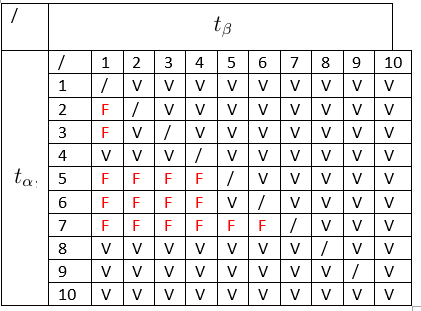
\includegraphics[scale=1]{img/TaxBad}
	\caption{\label{BadTax} Toutes les violations pour $\varphi$}
\end{figure}

Nous avons choisi $fv_1$ comme variable fraiche pour $t_2$. Bien que ce soit une variable fraiche, nous savons plusieurs choses à son propos. En effet nous savons les choses suivantes:
\begin{enumerate}

\item $I(t_1.Taxe)=0$ donc $I'(t_2.Taxe)>0$, i.e $fv_1>0$ car $I(t_1.Revenu)<I(t_2.Revenu)$
\item $I(t_4.Taxe)=3$ donc $I'(t_2.Taxe)<3k$, i.e $fv_1<3k$ car $I(t_2.Revenu)<I(t_4.Revenu)$

\end{enumerate}

Nous avons assigné une variable fraiche $fv_1$ comme valeur pour $t_2.Taxe$ mais nous savons quand même que $0<fv_1<3k$ i.e $fv_1 \in ]0,3k[$ grâce à 1 et 2. Nous pouvons utiliser la même logique pour connaitre les valeurs possible pour les autres variables fraiches. Nous pouvons dire que $fv_2 = fv_1$, $3k<fv_3<21k$, $fv_4 = fv_3$ et $fv_3<fv_5<21k$. Maintenant que nous avons identifié les valeurs erronées ainsi qu'un ensemble de valeurs pour remplacer les variables fraiches, il reste à savoir quelle valeur finale on peut prendre. Pour cela nous avons plusieurs solutions possibles.\\
\end{myexample}
\begin{itemize}
	\item Prendre une valeur de $\dom(A)$. C'est la solution envisagée dans le principal article de référence que nous utilisons. Il ne sera pas toujours possible de prendre une valeur dans le domaine, par exemple il n'y a pas de valeur dans le $dom(Taxe)= \{0,3k,21k,40k\}$ qui puisse satisfaire la condition $fv_1$. Dès lors, dans le cas où aucune valeur de dom(A) n'est attribuable à la variable fraiche, celle-ci est conservée dans la base de données. Cette pratique n'est pas la plus logique puisque même si nous avions une valeur dans $\dom(Taxe)$ qui puisse satisfaire $fv_1$, il y a plusieurs valeurs en dehors de $\dom(Taxe)$ qui sont tout aussi correctes.
	\item Prendre une valeur aléatoire mais respectant les conditions sur la variable fraiche. C'est une très mauvaise idée puisque nous avons une chance de s'éloigner de la vraie valeur. Cela peut impacter énormément l'ajout de tuples dans la relation après que la réparation soit effectuée. Ces nouveaux tuples malgré qu'ils soient corrects pourraient être perçus comme contenant des données erronées.
	\item Garder les variables fraiches dans la base de données tout en conservant les informations que l'on connait à propos de celles-ci. Si nous n'avons qu'une seule valeur possible alors nous privilégions cette valeur à $fv$. Cette solution est celle qui respectera le mieux l'intégrité des données. Le seul problème qu'apporte cette solution est que de nombreuses applications ne pourront plus fonctionner correctement avec des variables fraiches. De nombreux SGBD ne permettent pas de stocker ces variables. Les informations que l'on connait sur elles peuvent changer au fur et à mesure que la relation se remplit.
\end{itemize}

\begin{myexample}
\label{exampleDist}
Nous pouvons calculer le coût de réparation pour la relation de la table \ref{tableMain} en considérant les distances suivantes:\\

$$
\forall a \in dom(A) \ avec \ a \neq b.
\left\{
	\begin{array}{ll}
	   dist(a,a)=0\\
	   dist(a,b)=1\\
	   dist(a,fv)=1.5\\
	   dist(fv,fv)=1.5\\
	   dist(fv,b)=1\\
	\end{array}
\right.
$$

Lorsqu'on ne change pas la valeur, la distance est bien évidement égale à zéro. $dist(a,fv)$ soit être supérieure à $dist(a,b)$ pour privilégier les valeurs aux variables fraiches. $dist(fv,fv)$ représente le fait qu'on avait déjà une variable fraiche venant d'une réparation antérieure, et qu'on garde une variable fraiche. $dist(fv,b)$ représente le changement d'une variable fraiche venant d'une réparation antérieure par une valeur précise. Cela peut arriver lorsque l'on possède de plus amples informations sur la valeur fraiche,par exemple grâce à de nouveaux tuples dans la relation. Nous avons besoin que $dist(fv,fv) > dist(fv,b)$ pour favoriser la correction par une vraie valeur quand c'est possible. Dans l'exemple précédent, avec les valeurs susmentionnées, nous pouvons calculer un coût de réparation $\Delta(I,I')$ =$5*dist(a,a) + 5*dist(a,fv)$ = $7,5$.
\end {myexample}

\section{Variation sur les denial constraints}

Nous avons vu précédemment qu'une denial constraint peut être sur-raffinée, échouant donc dans la détection d'erreurs. Une DC peut aussi être sur-simplifiée ce qui conduit à considérer des données correctes comme étant erronées. Parce que les contraintes peuvent être imprécises et inexactes, nous avons besoin de les corriger. En modifiant ces contraintes, nous pouvons obtenir une meilleure réparation\\

\begin{myexample}
Par exemple prenons la DC suivante:

$$ \varphi = \{(Revenu,>),(Taxe,\leq) \} $$

La denial constraint $\varphi$ exprime le fait que si je reçois un revenu plus élevé qu'une autre personne, alors je dois payer un montant de taxe strictement plus élevé. Nous allons modifier $\varphi$ pour obtenir une nouvelle denial constraint $\varphi'$ en changeant le prédicat $(Taxe,\leq)$ en $(Taxe,<)$. Dès lors, maintenant $\varphi'$ exprime le fait que si je reçois un revenu plus élevé qu'une autre personne, alors je dois payer un montant de taxe plus élevé ou équivalent. Cela permet d'exempter de taxe plusieurs personnes ayant un Revenu faible, mais différent les uns des autres. 

$$ \varphi' = \{(Revenu,>),(Taxe,<) \} $$

Avec cette nouvelle contrainte, nous avons moins de violations détectées. Toutes les violations peuvent être trouvées à la figure $\ref{GoodTax}$. Les modifications que nous avons faites dans la table \ref{tableExample} sont:

\begin{table}[H]
	\centering
	\begin{tabular}{|c|c c c c c c c c c c|}
	\hline
	   & $t_1$ & $t_2$ & $t_3$ &$t_4$ &$t_5$ &$t_6$ &$t_7$ &$t_18$ &$t_9$ &$t_10$ \\
	\hline
	 Taxe & 0 & 0 & 0 & \textcolor{red}{$fv_1$} & 0 & 0 & 0 & 21k & 21k & 40k\\
	 \hline
	\end{tabular}
	\caption{\label{tableExample2} Example of repair with Tax}.
\end{table}


\begin{figure}
	\centering
	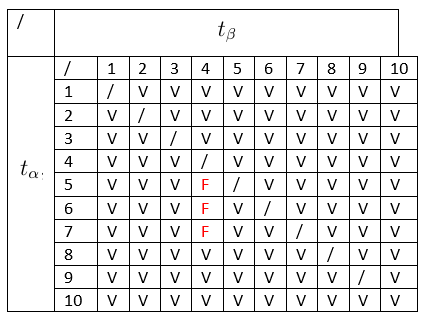
\includegraphics[scale=1]{img/TaxGood}
	\caption{\label{GoodTax} All the violation for $\varphi '$}
\end{figure}

Contrairement à la réparation de $\varphi$ qui proposait une correction avec 5 variables fraiches (voir table \ref{tableExample}), nous 'avons ici qu'une seule variable fraiche. De plus, nous savons certaines choses à propos de cette variable fraiche:

\begin{enumerate}

\item $t_1.Taxe=0$ donc $f(t_4).Taxe \geq 0$ car $t_1.Revenu < t_4.Revenu$
\item $t_5.Taxe=0$ donc $f(t_4).Taxe \leq 0$ car $t_4.Revenu < It_5.Revenu$

\end{enumerate}

Nous avons donc $0 \leq fv_1 \leq 0$, dès lors la seule valeur possible pour remplacer $fv_1$ est $fv_1 = 0$. Nous avons donc un coût de réparation de $\Delta(I,I') = 1$ en reprenant les valeurs de distance de l'exemple \ref{exampleDist}.

\end{myexample}

Nous voyons donc que la modification de la contrainte conduit à un coût de réparation plus faible. Mais modifier une contrainte doit aussi avoir un coût. En effet , si on ne donne pas de coût à la modification d'une contrainte, il suffirait de sur-raffiné toutes nos contraintes pour détecter moins de violations et donc faire moins de modifications. Nous allons aussi considérer que nous n'ajoutons pas DC ni n'en retirons de $\Sigma$ pour obtenir $\Sigma'$ et donc $|\Sigma| = |\Sigma'|$.\\

Nous devons désormais définir une marche à suivre concernant les variations de DC. Nous devons trouver un moyen de définir un coût de variation. Considérons le treillis tel qu'illustré à la figure \ref{treillis} pour un attribut $A$ de $S$. Chaque nœud du treillis représente un prédicat différent pour $A$, donc $A$ associé à un opérateur, un des éléments de l'ensemble puissance de $OP$. Descendre dans une branche du treillis consiste à ajouter un élément de $OP$ à l'opérateur. Par exemple passer de $(A,<)$ à $(A,\leq)$ consiste à ajouter l'opérateur $=$ à $\{ < \}$. Lorsque l'on monte dans le treillis, on retire un élément de $OP$ à l'opérateur. Par exemple, passer de $(A, \geq)$ à $(A,=)$ consiste à retirer l'opérateur $>$ à $\{ >,= \}$.\\

\begin{figure}
	\centering
	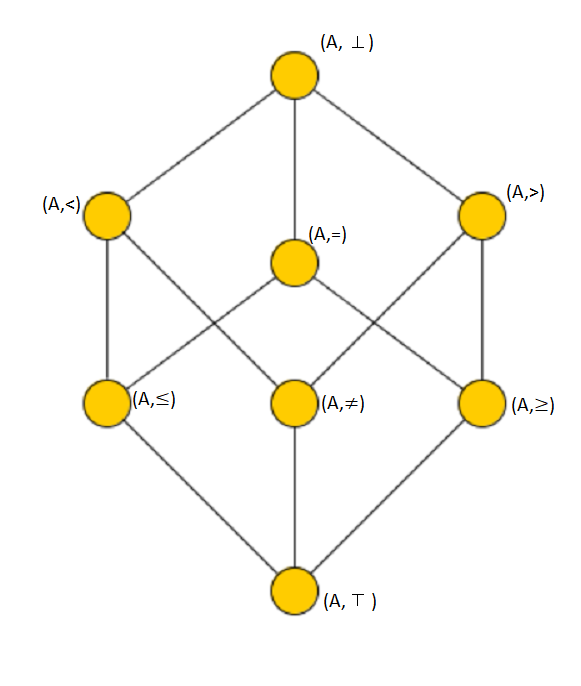
\includegraphics[scale=0.5]{img/treillis}
	\caption{\label{treillis} Treillis pour un prédicat d'attribut $A$}
\end{figure}

% déplacer section suivante$
Nous devons modifier nos DC de telle manière qu'une contrainte sur-raffinée ou sur-simplifiée ne le soit plus. Si une DC est sur-raffinée, nous devons descendre dans le treillis. En effet , plus on descend dans le treillis, plus le prédicat sur l'attribut $A$ sera faible, i.e la DC sera faible. A l'inverse, si une DC est sur-simplifiée; nous devons monter dans le treillis. En effet plus nous montons dans le treillis, plus le prédicat sur l'attribut $A$ sera fort, i.e la DC sera plus forte. Plus nous changeons de prédicats, plus le \emph{coût de variation des contraintes} sera important. Le \emph{coût de variation des contraintes} se définit comme tel: 

\begin{mydef}
Soit $\Sigma$ un ensemble de DC sur un ensemble $S$. Pour une variante $\Sigma '$ de $\Sigma$, la fonction de calcul du \emph{coût de variations des contraintes} de $\Sigma$ est:

$$\Theta (\Sigma,\Sigma ') = \sum_{\varphi in \Sigma} edit(\varphi,\varphi ')$$

\hspace*{2cm} avec $\varphi '$ une variante de $\varphi$ et $edit(\varphi,\varphi ')$ est le coût pour changer $\varphi$ en $\varphi'$.
\end{mydef}

La fonction $edit(\varphi , \varphi ')$ qui indique le coût pour changer $\varphi$ en $\varphi'$ est défini comme étant:

\begin{mydef}
$$
 edit(\varphi, \varphi') = \sum_{A \in S} path(\varphi(A),\varphi'(A))$$
 
avec $path(\varphi(A),\varphi'(A))$ le coût du chemin emprunté dans le treillis.
\end{mydef}

Si nous considérons notre treillis comme un graphe, il reste maintenant à trouver le poids de chacun des arcs de ce graphe.

\subsection{Parcours dans le treillis}

	Maintenant que nous avons défini le poids de variation des contraintes, regardons le coût pour se déplacer dans le treillis. Soit $\varphi$ une DC sur $S$ et $\varphi'$ une variante de $\varphi$. Soit $A$ un attribut sur $S$. Le cout pour passer de $\varphi(A)$ à $\varphi'$, i.e la valeur de $path(\varphi(A),\varphi'(A)$ est le coût du plus court chemin du treillis. Le treillis doit être vu comme un graphe pouvant être parcouru dans les deux sens. Le poids de chaque arc est de $c(A)$, $c(A)$ étant une valeur symbolisant la confiance qu'on accorde à la valeur de $A$. Si on n'a aucune connaissance sur la base de données, $c(A) =c(B)$ , pour tout $A,B \in S$.
	
\begin{myexample}
	Soit $\varphi = \{(Taxe,\leq),(Revenu,<) \}$ et $\varphi' = \{(Taxe,>)(Revenu,<) \}$ et c(A) =1.
	
	Pour passer de $(Taxe,\leq)$ à $(Taxe,>)$, un chemin possible est $(Taxe,\leq) \rightarrow (Taxe,<) \rightarrow (Taxe,\bot) \rightarrow (Taxe,>)$ et ce chemin à un coût de 3.
\end{myexample}

Par observation, on peut facilement se rendre compte que le plus court chemin du treillis est de longueur 3 maximum. Dans les sous-sections qui suivent, nous verrons qu'il sera important de limiter nos candidats, ce qui modifiera éventuellement le poids de certains arcs.

\subsection{Limitation des candidats}


Dans notre treillis, nous avons 8 nœuds. Pour une DC sur un ensemble $S$ de taille 1, nous avons 8 différentes variantes de DC. Pour un ensemble $S$ de taille $n$ nous avons $8^n$ variations. Ce nombre est très important et envisager toutes les variations de contraintes serait coûteux en terme de complexité. Si le calcul d'une variation se fait en $O(1)$ alors considérer toutes les variantes possible est en $O(8^n)$. Si l'ensemble $\Sigma$ de contraintes est de taille $l$, puisqu'il faut considérer toutes les variantes pour chaque DC $\varphi \in \Sigma$, la complexité serait de $O((8^n)^l)$ Nous avons donc besoin de limiter le nombre de variations à considérer. Pour ce faire, nous allons utiliser des propriétés sur les DC pour limiter le nombre de contraintes à considérer.\\

Nous savons déjà par le chapitre précédent que les contraintes triviales sont inutiles. En effet, une contrainte triviale sera toujours vraie et donc considérera tous les tuples comme étant corrects. Le Lemme \ref{trivialLemma} nous permet de rejeter toutes les DC dont au moins un des prédicats est de la forme $(A,\bot)$.\\

Nous avons également besoin que la denial constraint soit satisfiable. Si une DC n'est pas satisfiable alors elle possède uniquement des prédicats avec l'opérateur $\top$ ou $=$. Nous pouvons donc rejeter toutes les DC ne possédant aucun opérateur parmi $\{ \leq,\geq,\neq,<,> \}$\\

\subsection{Denial constraints maximales}

Nous avons besoin également que les DC soit \emph{maximales}. Dans \cite{main} ils définissent une DC maximale comme étant:

\begin{mydef}
 La variante $\varphi'$ d'une DC $\varphi$ est dite \emph{maximale} si  $\varphi \preceq \varphi'$ \footnote{voir définition du raffinement chapitre \ref{RaffinementSection}} est qu'il n'existe pas de DC $\varphi''$ tel que $\varphi' \preceq \varphi'$ et que $edit(\varphi,\varphi'') = edit(\varphi,\varphi')$
\end{mydef}

\begin{myprop}\cite{main}
\label{maxprop}
Soit $\varphi$ une DC sur $S$. Soit $\varphi'$ une variante de $\varphi$ sur $S$. Pour chaque attribut $A$ de $S$ tel que $\varphi(A) = \{ \top, =, <, > \}$, si $\varphi'(A) \in \{\neq,\leq,\geq \}$ alors $\varphi'$ n'est pas maximal.

\end{myprop}

Cette propriété vient de la définition de $Imp(\varphi)$. Soit $\varphi_1, \varphi_2$ deux DC sur $S$ Soit une relation $I$ sur $S$. Pour deux tuples $s,t \in I$ et un attribut $A$ de $S$, si $\varphi_1 \in Imp(\varphi_2)$ alors $s.A \Theta_1 t.A$ implique $s.A \Theta_2 t.A$ avec $\Theta_1 = \varphi_1(A)$ et $\Theta_2 = \varphi_2(A)$. Les opérateurs $\leq$, $\geq$ et $\neq$ sont les seuls opérateurs qui impliquent d'autres opérateurs qu'eux même comme on peut le voir à la table \ref{operatorTable}(c'est également le cas pour l'opérateur $\top$, mais celui-ci est exclu de la propriété).\\

Grâce à cette propriété, nous savons maintenant qu'il est inutile de considérer toutes les insertions \footnote{Par insertion de prédicats, comprenons ici que nous passons de $\varphi(A) = \top$ à $\varphi(A) \neq \top$} de prédicats possibles. Nous avons seulement besoin d'insérer des prédicats avec les opérateurs $\{<,=,>\}$ lorsque que l'on considère les variantes de $\varphi$. Illustrons cela avec un exemple. 
\begin{myexample}
Nous allons prendre deux DC sur la relation de la table \ref{tableMain}:
$$ \varphi_1 : \{(Nom,=),(Revenu,=),(Numtel,\neq) \}$$

$$ \varphi_2 : \{(Nom,=),(Revenu,\leq),(Numtel,\neq) \}$$

\end{myexample}

Nous savons que $\leq \in Imp(=)$ (voir table \ref{operatorTable}) donc nous avons $\varphi_2 \preceq \varphi_1$. Grâce à la propriété \ref{maxprop}, $\varphi_2$ n'est pas une denial constraint maximale parce qu'elle contient l'opérateur $\leq$. Dans ce scénario, nous pouvons calculer un coût de réparation pour l'attribut $NumTel$ de 7 pour la DC $\varphi_2$ et la DC $\varphi$ aura un coût de réparation de $Numtel$ de valeur 3.

\begin{table}[H]
	\parbox{.45\linewidth}{
	\centering
	\begin{tabular}{|c|c c c|}
	\hline
	    & Nom & NumTel & Revenu\\
	\hline
	 t1 & Ayres & \color{red}564-389 & \color{red}22k\\
	 t2 & Ayres & \color{red}564-389 & 22k\\
	 t3 & Ayres & 564-389 & 22k\\
	 t4 & Stanley &\color{red} 930-198 &\color{red}24k\\
	 t5 & Stanley &\color{red} 930-198 & 24k\\
	 t6 & Stanley & 930-198 & 24k\\
	 t7 & Dustin & \color{red}824-870 & \color{red}100k\\
	 t8 & Dustin & \color{red}824-870 & 100k\\
	 t9 & Dustin & 824-870 & 100k\\
	 t10 & Dustin & \color{red}824-870 & \color{red}100k\\
	 \hline
	\end{tabular}
	\caption{Correction avec $\varphi_2$: 7 changement nécessaire dans la colonne $NumTel$}.
	}
	\hfill
	\parbox{.45\linewidth}{
	\centering
	\begin{tabular}{|c|c c c|}
	\hline
	    & Nom & NumTel & Revenu\\
	\hline
	 t1 & Ayres & 322-573 & 21k\\
	 t2 & Ayres & \color{red} 564-389 & 22k\\
	 t3 & Ayres & 564-389 & 22k\\
	 t4 & Stanley & 868-701 &23k\\
	 t5 & Stanley & \color{red} 930-198 & 24k\\
	 t6 & Stanley & 930-198 & 24k\\
	 t7 & Dustin & 179-924 & 25k\\
	 t8 & Dustin & \color{red} 824-870 & 100k\\
	 t9 & Dustin & 824-870 & 100k\\
	 t10 & Dustin & 387-215 & 150k\\
	 \hline
	\end{tabular}
	\caption{Correction avec $\varphi_1$ : seulement 3 changements sont nécessaires.}.
	}
\end{table}



Nous voyons que la DC raffinée a un coût de réparation plus faible. Ce n'est pas une coincidence puisque le Lemme suivant existe: \cite{main}

\begin{mylemma}
 Soit $\Sigma$ un ensemble de DC sur $S$ et $I$ une relation sur $S$. Soit 2 variantes de $\Sigma$ noté $\Sigma_1,\Sigma_2$ et $\Sigma_2$ est un raffinement de $\Sigma$. Si $\Sigma \preceq \Sigma_1$ et $\Sigma_1 \preceq \Sigma_2$ alors $\Delta(I,I_1) \geq \Delta(I,I_2)$ avec $I_1$ la relation résultante de la réparation avec $\Sigma_1$ et $I_2$ la relation résultante de la réparation avec $\Sigma_2$.
\end{mylemma}

Comme conséquence à ce Lemme, tous les ensembles de denial constraint $\Sigma$ qui ne sont pas maximals ne donneront pas la meilleure réparation.

\subsection{Limitation par bornes}

Nous avons vu précédemment que pour une seule DC, nous avions $8^{|S|}$ variantes possibles (voir treillis à la figure \ref{treillis} ). Nous avons donné des pistes pour limiter le nombre de candidats. Pour continuer dans cette lancée, nous allons déterminer deux bornes entre lesquelles le coût de la réparation la moins coûteuse se trouve. Nous avons la borne inférieure notée $\delta_l(\Sigma,I)$ et la borne supérieure notée $\delta_u(\Sigma,I)$. Nous savons que le coût de réparation $\Delta(I,I')$ pour la relation $I$ sur $S$ avec l'ensemble de DC $\Sigma$ sera situé entre les deux bornes i.e $\delta_l(\Sigma,I) \leq \Delta(I,I') \leq \delta_u(\Sigma,I)$. L'idée étant qu'on puisse calculer les deux bornes très rapidement, là où $\Delta(I,I')$ ne peut être calculer qu'après avoir essayer la réparation. Considérons la propriété suivante:

\begin{myprop}
\label{boundRemove}
	Soit deux ensemble de denial constraints $\Sigma_1$ et $\Sigma_2$ pour une relation $I$ sur $R$, si $\delta_u(\Sigma_1,I) < \delta_l(\Sigma_2,I)$ alors $\Sigma_2$ n'est pas un bon candidat et peut être ignoré.
\end{myprop}


\begin{proof}~\\
\hspace*{0.5cm} Soit $I$ une relation sur $S$ et $\Sigma$ un ensemble de DC.

Soit $\Sigma_1 , \Sigma_2$ deux ensemble de DC, variantes de $\Sigma$.

Soit $I_1 , I_2$ deux relations résultantes de la réparation de $I$ avec les ensembles de DC $\Sigma_1, \Sigma_2$ respectivement.

Par hypothèse nous avons $\delta_l(\Sigma_1,I)$ < $\Delta(I,I_1)$ < $\delta_u(\Sigma_1,I)$ et $\delta_l(\Sigma_2,I)$ < $\Delta(I,I_2)$ < $\delta_u(\Sigma_2,I)$ et $\delta_u(\Sigma_1,I)$ < $\delta_l(\Sigma_2,I)$.

Dès lors nous avons $\delta_l(\Sigma_1,I)$ < $\Delta(I,I_1)$ < $\delta_u(\Sigma_1,I)$ < $\delta_l(\Sigma_2,I)$ < $\Delta(I,I_2)$ < $\delta_u(\Sigma_2,I)$.

Alors par transitivité  $\Delta(I,I_1)$ < $\Delta(I,I_2)$. $I_2$ est une réparation plus couteuse que $I_1$ i.e $\Sigma_1$ est un meilleur candidat que $\Sigma_2$.
\end{proof}

Cela veut dire que si la pire borne (borne supérieure) de la réparation de $\Sigma_1$ est moins bonne que la meilleure borne (borne inférieure) de la réparation de $\Sigma_2$ alors $\Sigma_1$ sera un meilleur ensemble DC pour la réparation que $\Sigma_2$ et donc $\Sigma_2$ peut être abandonnée. C'est intéressant pour l'élaboration d'un algorithme cherchant à trouver le meilleur ensemble de contraintes. En effet, si le calcul de ces bornes est moins couteux que le calcul du cout de réparation $\Delta(I,I')$ alors on peut réduire la complexité de cet algorithme.


\subsubsection{Graphe de conflits}

Maintenant, nous allons introduire le \emph{graphe de conflits} qui peut représenter les violations dans une relation $I$ sur $S$. Dans un premiers temps, nous avons besoins de trouver l'ensemble de toutes les violations et ensuite obtenir nos deux bornes grâce à cet ensemble. On définition l'\emph{ensemble des violations} comme étant: \cite{main}

\begin{mydef}
 L'\emph{ensemble des violations} $viol(I,\varphi) = \{ (s,t) | (s,t) \not\models \varphi $ avec $ s,t \in I \}$ est un ensemble de couple de tuples qui viole $\varphi$.L'ensemble de violation de $\Sigma$ est $viol(I,\Sigma) = \cup_{\varphi \in \Sigma}viol(I,\varphi)$.
\end{mydef}

\begin{figure}
 \centering
 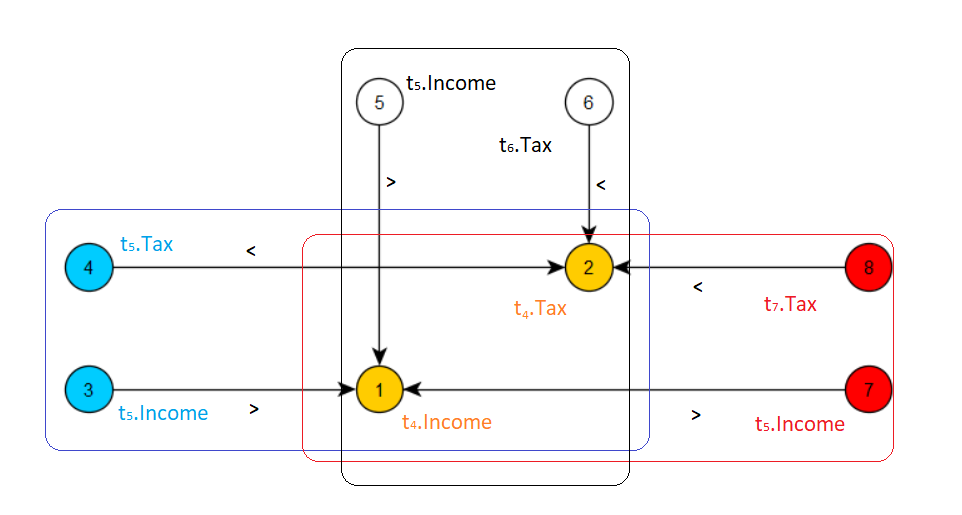
\includegraphics[scale=0.8]{img/grapht4.png}
 \caption{\label{grapht4} Graphe de conflits pour $\varphi$}
\end{figure}

\begin{mydef}
	L' \emph{ensemble cellules impliquées dans les violation} noté $cell(\varphi)$ est définie comme étant $cell(\varphi) = \{t.A,s.A|s,t \in I, (s,t) \in viol(I,\varphi), \varphi(A) \neq \top \}$. Les cellules de deux tuples $s,t \in I$ impliquées dans les violations de $\varphi$ est définie par $cell(s,t\varphi) = \{t.A,s.A|s,t \in I, \varphi(A) \neq \top \}$.
\end{mydef}

Avec le graphe de conflits $G$ nous pouvons représenter les violations dans la relation $I$. Pour chaque $(s,t) \in viol(I,\varphi)$ il y a un arc pour $cell(s,t,\varphi)$ dans G. Une bonne réparation $I'$ consiste à réparer la base de données de telle manière à ce que tout les arcs soient supprimés. Dès lors après une réparation, le graphe est vide.

\begin{myexample}
Prenons un exemple sur la table \ref{tableMain} ainsi qu'une DC que nous avons déjà utilisé auparavant:

$$\varphi' =\{(Revenu,>),(Taxe,<) \})$$

Pour notre relation, l'ensemble des violations est (voir figure \ref{GoodTax}):
 $$ viol(I,\varphi') = \{ (t_5,t_4),(t_6,t_4),(t_7,t_4) \}$$

Dans notre graphe, $(t_5,t_4) \in viol(I,\varphi')$ est représenté par $cell(t_5,t_4;\varphi')$ qui est égale à $\{ t_5.Revenu, t_4.Revenu, t_5.Taxe, t_4.Taxe\}$. Nous voulons éliminer les conflits, ce qui se traduit par éliminer les arcs du graphe. Introduisons d'abord deux Lemmes et une définition: \cite{main}
\end{myexample}
	%% problems here%%
\begin{mydef}
	On note $ \min_{a} dist(t.A,a) $ le poid d'un arc t.A, i.e, le coût minimum qui devrait être payé pour réparer t.A avec une valeur $a$.
\end{mydef}

\begin{mydef}
	$\mathbb{V}(G)$ est la \textbf{couverture de poids minimum} du graphe G correspondant à $\Sigma$ avec le poids
	$$||\mathbb{V*(G)}|| = \sum_{t.A \in \mathbb{V}(G)} min_{a} dist(I(t.A),a)$$
\end{mydef}

\begin{mylemma}
	Soit $I$ une relation sur $S$. Pour n'importe quelle réparation $I'$ de $I$, i.e, $I' \models \Sigma$, nous avons $\Delta(I,I') \leq ||V*(G)||$. 
\end{mylemma}

\begin{mydef}
	Soit $I$ une relation sur $S$. Soit $\Sigma$ un ensemble de DC. Soit $s$,$t$ deux tuples de $I$. Nous définissons degré de $\Sigma$ noté $Deg(\Sigma)$ comme étant : $$Deg(\Sigma) = \sum_{\varphi \in \Sigma} |cell(s,t,\varphi)|$$
\end{mydef}

%Computing $\mathbb{V}$ is a NP-Hard problem so we need to approximate it. We'll consider an constant factor-f approximation of $\mathbb{V}$ which is $\frac{||\mathbb{V}(G)||}{||\mathbb{V}*(G)||} \leq f$. where f is the maximum degree of hyperedges and $||\mathbb{V}(G)||$ is an approximation of $||\mathbb{V}*(G)||$.

Dans \cite{main} ils définissent la borne supérieure et la borne inférieure du coût de réparation comme étant:
$$ \delta_l(\Sigma,I) = \frac{||\mathbb{V}(G)||}{Deg(\Sigma)}$$
$$ \delta_u(\Sigma,I) = \sum_{t.A \in \mathbb{V}(G)} dist(I(t.A),fv)$$

Si nous revenons à notre example et que nous supposons que nous avons les distances suivantes :

$$
\forall a \in dom(A) \ avec \ a \neq b.
\left\{
	\begin{array}{ll}
	   dist(a,a)=0\\
	   dist(a,b)=1\\
	   dist(a,fv)=1.5\\
	   dist(fv,fv)=1.5\\
	   dist(fv,b)=1\\
	\end{array}
\right.
$$

Donc si chaque arc a un poids de 1 (=$ dist(a,b)$) et si nous posons $\mathbb{V}(G)$ = $\{t_4.Tax \}$ nous avons $||\mathbb{V}(G)||$ = 1. Nous avons aussi $Deg(\Sigma)$ = 4, donc en utilisant les formules pour le calcul des bornes supérieure et inférieure: $\delta_l(\Sigma,I)$=$\frac{||\mathbb{V}(G)||}{Deg((\Sigma)}$ = $\frac{1}{4}$ = 0.25 and $\delta_u(\Sigma,I) = \sum_{t.A \in \mathbb{V}(G)} dist(I(t.A),fv)$ = $dist(a,fv)$=1.1 .

%%problem end%%

\subsection{Coût dans le treillis}

Nous pouvons donc modifier une DC $\varphi$ en modifiant ses prédicats. Nous avons vu précédemment que les opérateurs peuvent être représenter dans un treillis et modifier l'opérateur consiste à se déplacer dans le treillis. Le coût dépend donc du nombre d'arcs parcourus dans le treillis. Nous verrons dans cette sous-section quel est le poids pour chacun de ces arcs.\\

Il est possible de représenter le treillis comme à la figure \ref{treillisGraph}. Chaque couleur représente un type de changement. Par exemple chaque arc orange représente un changement depuis l'opérateur $\{ \} \equiv \bot$ vers un élément de $OP$ de taille 1. Discutons maintenant du poids que l'on peut donner à chacun de ces arcs.

\begin{mydef}

	Soit $I$ une relation sur $S$. Soit $\mathbb{T}$ un treillis pour un attribut $A \in S$. On note $w(a,b)$ le poids d'un arc de $\mathbb{T}$ depuis un élément de $OP$ de taille $a$ vers un élément de $OP$ de taille b.

\end{mydef}


\begin{figure}
	\centering
	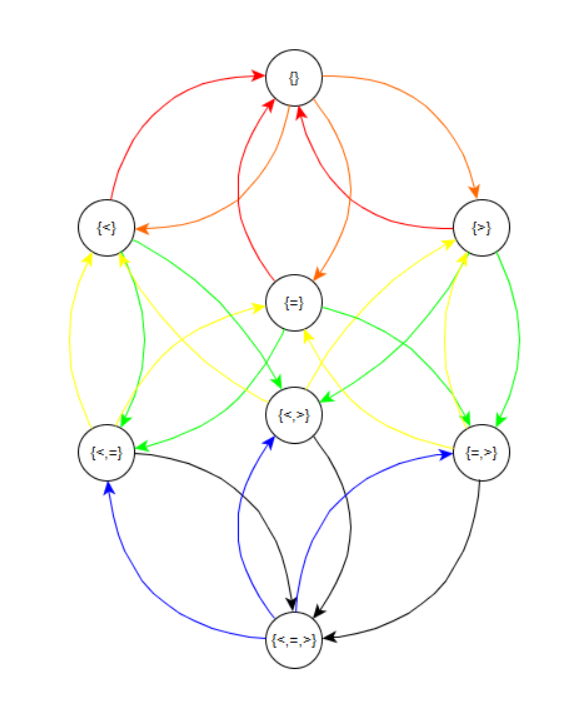
\includegraphics[scale=0.655]{img/treillisGraph}
	\caption{\label{treillisGraph} Chaque types de transition aura son propre poids.}
\end{figure}


Nous avons vu précédemment qu'une DC ne doit pas contenir l'opérateur $\bot$ car sinon la DC est triviale (voir Lemma \ref{trivialLemma}). De ce fait nous pouvons dire:

\begin{itemize}
	\item Il ne faut pas transformer un opérateur en $\bot$. Les arcs allant vers $\bot$ , i.e les arcs rouges dans la figure \ref{treillisGraph}, ne doivent jamais être empruntés. Pour cela, le poids de ces arcs sera $w(1,0)= + \infty$
	\item Une DC ne devrait jamais avoir de prédicat dont l'opérateur est $\bot$. Si c'est le cas, il est nécessaire de corriger ce prédicat. Pour aider à la correction, nous posons $w(0,1) < 0$, dès lors emprunter un arc orange ne coute rien, c'est même positif et donc on encourage à faire cette modification. On force ainsi la correction de tels prédicats.
\end{itemize}

Nous avons également vu que si une DC n'est pas maximale, alors elle ne donnera pas la meilleure réparation. Il faut donc sanctionné les transitions qui partent d'un prédicat maximal vers un prédicat non maximal. Par la propriété \ref{maxprop}, nous savons que les prédicats qui contiennent les opérateurs $\leq, \geq$ ou $\neq$ ne sont pas maximals. Pour encourager à rendre une DC maximale, nous poserons $w(1,2)$ = + $\infty$ et $0 < w(2,1) <\alpha$ avec $\alpha$ un seuil que nous devrons définir plus tard.

Il nous reste à évaluer $w(2,3)$ et $w(3,2)$. $w(3,2)$ représente une insertion de prédicat tandis que $w(2,3)$ est une suppression de prédicat. A priori, il n'y a aucune raison de mettre un poid particulier sur ces transitions. Nous poserons que $0 < w(3,2)  = w(2,3) < \alpha$.

\subsection{Variation d'un ensemble de contraintes}

Nous avons jusqu'à présent abordé le sujet de la variation d'une seule contrainte. Pour faire varier un ensemble de contraintes $\Sigma$, il suffit d'appliquer le même raisonnement à au moins une des DCs de $\Sigma$. Mais nous devons statuer si on peut ajouter des DC ou même en supprimer. Nous déciderons d'aller dans le même sens que l'article sur lequel nous nous sommes initialement basés \cite{bcss} et donc nous n'ajouterons pas de DC ni n'en retirerons. Retirer une DC diminue le nombre d'erreurs détectées (l'ensemble des DC est sur-raffiné)et on peut supposer que chaque DC avait un sens lors de sa création (mais peut évidement être imprécis). L'ajout de DC est bien plus compliqué a mettre en oeuvre et on peut rapidement obtenir des DC qui n'ont pas de sens et qui détecteraient des erreurs qui ne le sont pas (l'ensemble de DC est sur-simplifié).

Puisque nous avons décidé de ne pas supprimer des DCs dans un ensemble de DC $\Sigma$, nous devons faire attention à la manière dont nous modifions $\Sigma$. Si cet ensemble contient au moins deux DC et qu'on modifie une des contraintes jusqu'à ce qu'elle soit identique à une autre, alors ça revient à faire une suppression.

\begin{myexample}
Soit $S$ = $\{A,B,C\}$
Prenons $\Sigma_1 = \{ \varphi_1= \{(A,<),(B,\neq) \} \varphi_2= \{(A,<),(C,\neq) \}\}$ et la variation $ \Sigma_2 = \{ \{(A,<),(B,\neq) \} ,\{(A,<),(B,\neq) \}\}$
nous voyons que la variation contient deux fois la même DC, et donc on peut réécrire $ \Sigma_2 = \{ \{(A,<),(B,\neq) \}\}\}$ ce qui équivaut à une suppression.

\end{myexample}

Notons qu'il est possible de faire des variations inutiles :

\begin{myexample}

Reprenons $S$ = $\{A,B,C\}$
et $\Sigma' = \{ \varphi_1= \{(A,<),(B,\neq) \} \varphi_2= \{(A,<),(C,\neq) \}\}$ et la variation $\Sigma' = \{ \varphi_1'= \{(A,<),(C,\neq) \} \varphi_2'= \{(A,<),(B,\neq) \}\}$ , les deux DC ont été modifiés mais nous avons le même ensemble!
\end{myexample}
\section{$\theta$-tolerant model}

Dans cette section nous allons enfin aborder le \emph{modèle de réparation $\theta$-tolérant}. $\theta$ représente ici un seul de variation sur l'ensemble des contraintes $\Sigma$, nous ne voulons donc pas une variante de contraintes dont le coût serait plus grand que $\theta$ : $\Theta(I,I') \leq \theta$. L'idée est d'éviter le sur-raffinement et donc d'éviter de laisser certaines données erronées. Afin d'éviter la sur-simplification, nous utilisons le principe du changement minimum. Nous avons donc besoin d'une relation réparée $I'$ de la relation originale $I$ et minimisant le coût de réparation $\Delta(I,I')$.\\

Trouver la meilleure réparation suivant le modèle $\theta$-tolérant, i.e trouver la réparation de coût minimum est un problème de la classe NP-difficile. La classe de problèmes NP-difficile est une classe dont les problèmes sont au moins aussi difficile que les problèmes les plus difficiles de la classe NP \footnote{Les problèmes NP sont des problèmes dont une solution peut être vérifiée comme étant bonne en un temps polynomial}. Nous devons donc retenir ici que ce n'est pas possible de résoudre la réparation $\theta$-tolérante en un temps polynomial. L'approche naïve est de récupérer toutes les variantes $\Sigma'$ de $\Sigma$ et de ensuite calculer $\Theta(I,I')$  avec $I'$ la relation résultante de la réparation suivant les DC de $\Sigma'$. Si $\Theta(I,I') \leq \theta$, on calcule le coût de réparation. Ensuite on compare le coût de la réparation $I'$ pour chaque $\Sigma'$ et on garde la réparation la moins coûteuse. Cette méthode est évidement très haute en complexité.\\

Nous avons vu qu'on remplaçait chaque donnée erronée par une variable fraiche $fv$ puis nous essayons de remplacer certaines de ces variables fraiches par des vraies valeurs. Plus une réparation privilégies les vraies valeurs aux valeurs fraiches, plus elle aura de chance de minimiser le coût de réparation.\\

Maintenant, considérons $\mathbb{D}$ = $\Sigma_1 ' * \Sigma_2' * ... \Sigma_{|\Sigma|}'$ où chaque $\Sigma_i' \in \mathbb{D}$ est une variante de $\Sigma$ obtenu par variations. Considérons que ces variantes sont limitées par $\theta$, donc nous avons $\Theta(\Sigma,\Sigma') \leq \theta$. L'algorithme \ref{theta} retourne la meilleure relation $I_{min}$ de l'ensemble des contraintes $\Sigma_{min}$. L'algorithme est simple: pour chaque $\Sigma_i$ , si la borne inférieure est plus petite que la borne supérieure (voir la propriétés \ref{boundRemove}), nous mettons à jour la valeur de $\delta_{min}$ car une meilleure réparation $I_i$ a été trouvée. \\

\IncMargin{1em}
\begin{algorithm}
\label{theta}

	\DontPrintSemicolon
  \caption{$\theta$-TolerantRepair$(\mathbb{D},\Sigma,I)$}
  \LinesNumbered
    \SetKwInOut{Input}{Entréé}
    \SetKwInOut{Output}{Sortie}

   % \underline{$\theta$-TolerantRepair} $(\mathbb{D},\Sigma,I)$\;
    \Input{Relation $I$, ensemble de DC $\Sigma$, ensemble $\mathbb{D}$ de variantes de DC bornées par $\theta$ }
    \Output{Une relation réparée $I_{min}$}
    $\delta_{min}$ = $\delta_u(\Sigma,I)$\;

	\Pour{chaque variante de contrainte $\Sigma_i \in \mathbb{D}$}{
    	\Si{$\delta_l (\Sigma_i,I) \leq \delta_{min}$}
    		{
    		$I_i$ = DATAREPAIR($\Sigma_i,I,\mathbb{V}(G_i),\delta_{min}$)\;
    		\Si{$\Delta(I,I_i) \leq \delta_{min}$}
    		{$\delta_{min}$ = $\Delta(I,I_i)$\;
    		$I_{min}$ = $I_i$\;}
    		}   		
    		
	}
	\Return $I_{min}$

\end{algorithm}\DecMargin{1em}

\begin{myexample}

Pour prendre un exemple, imaginons que nous avons un $\theta = \frac{?}{?}$ et un ensemble de variations de contraintes $\mathbb{D}$ = $\{\Sigma_1,\Sigma_2\}$ avec comme premier ensemble $\Sigma_1$ = $\{\varphi'\}$ et comme second ensemble $\Sigma_2$ = $\{\varphi''\}$ avec:
$$ \varphi' = \{(Revenu,>),(Taxe,<) \} $$
$$ \varphi'' = \{(Revenu,>),(Taxe,=) \} $$

Nous avons déjà fait le graphe de conflit pour la DC $\varphi'$ que l'on retrouve à la figure \ref{grapht4} et on sait également que $\delta_u(\Sigma_1,I) =1.1$\\

Pour $\Sigma2$ nous obtenons le graphe de conflit de la figure \ref{graphSigma2} (et les violations se retrouvent à la figure \ref{EqualTax}) avec $\mathbb{V}(G_2)$ = $\{ t_2.Tax,t_3.Tax,t_5.Tax,t_6.Tax,t_7.Tax\}$. Nous $Deg(\Sigma_2)$ = $Deg(\varphi')$ \footnote{Même raisonnement que précédement, nous avons 4 cellules impliquées.}, donc nous avons $\delta_l(\Sigma_2,I)$= $\frac{6}{2}$ = 1,5. Rappelons tout de même que $\delta_u(\Sigma_1,I)$ =1.1, donc nous avons $\delta_u(\Sigma_1,I) < \delta_l(\Sigma_2,I)$ ce qui signifie que nous pouvons ignorer $\Sigma2$ et donc ne pas appeler la fonction DATAREPAIR pour $\Sigma_2$. Nous parlerons de la fonction DATAREPAIR plus tard.



\begin{figure}
\centering
\hspace*{-1.8cm} 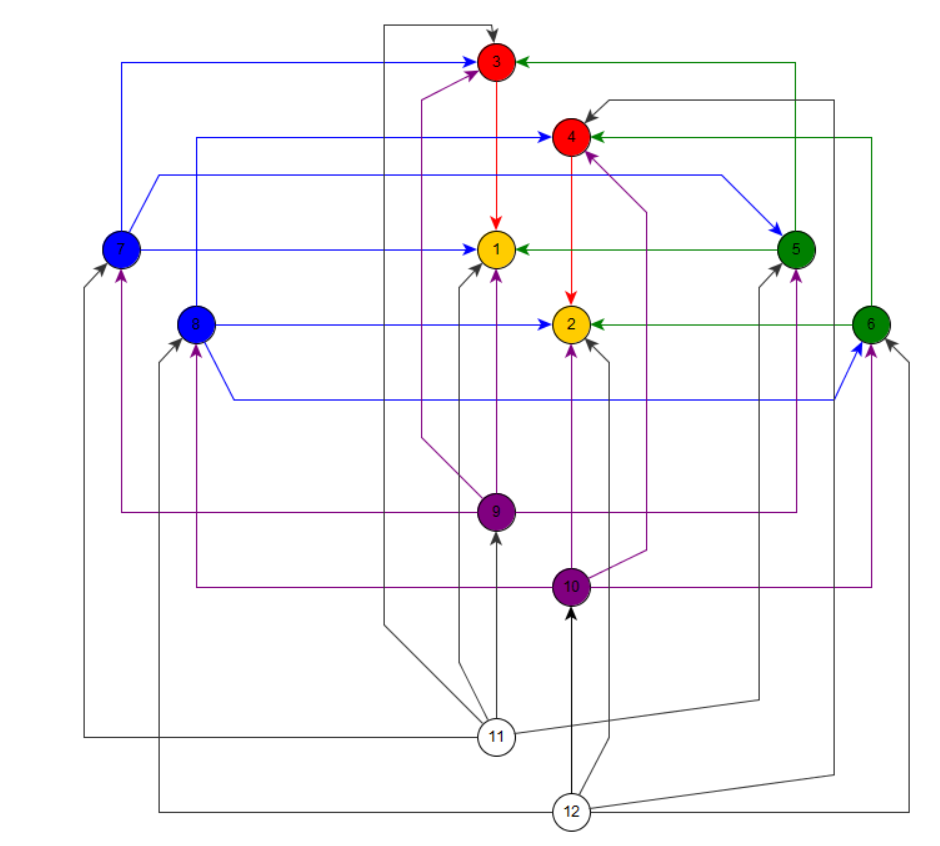
\includegraphics[scale=0.565]{img/graph2}
\caption{\label{graphSigma2}Graphe de conflit pour $\Sigma_2$ avec:}
	nombre pair pour les Taxe, nombre impair pour le Revenu. \\
	$t_1$ en jaune, $t_2$ en rouge, $t_3$ en vert,\\
	$t_4$ en bleu, $t_5$ en violet et $t_6$ en blanc.
\end{figure}

\begin{figure}
\centering
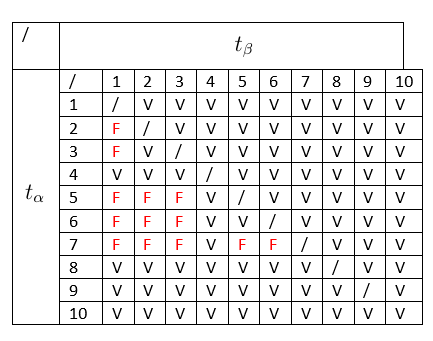
\includegraphics[scale=1]{img/TaxEqual}
\caption{\label{EqualTax} Toutes les violations pour $\varphi''$}
\end{figure}

\end{myexample}

Parlons maintenant de la complexité de l'algorithme. Disons que $l$ est le nombre de contraintes impliquées dans $\Sigma$ dès lors nous pouvons dire que la construction du graphe de conflits $G_i$ pour chaque $\Sigma_i \in \mathbb{D}$ est en $O(|I|^l)$. L'algorithme de réparation de données a une complexité en temps de $O(|I|^l)$ et l'algorithme \ref{theta} a une complexité en temps de $O(|I|^l|\mathbb{D}|)$. 

\section{Réparation au coût minimal}

Après avoir utilisé le modèle $\theta$-tolérant, nous connaissons enfin quel ensemble de denial constraints $\Sigma'$ (obtenu en faisant varier $\Sigma$) nous devons utiliser. Mais pour l'instant, nous n'avons pas encore vu comment effectuer la réparation. Nous avons seulement expliqué que chaque mauvaise donnée est remplacée par une variable fraiche et ensuite remplacée par une vraie valeur si possible. Dans cette section, nous allons nous concentrer sur la réparation de données en minimisant le coût et en se basant sur $\Sigma'$. Pour ce faire, nous allons devoir nous assurer que nous ne créons pas de nouvelle violation après avoir corrigé une donnée. Par exemple, si nous choisissons de changer la valeur de $t_5.Taxe$ à $22k$, nous réglons la violation sur $(t_5,t_4)$ que nous avions avec la denial constraint $\varphi$ = $\{ (Revenu,>)(Taxe,<)\} $. En changeant cette valeur de cette manière, on crée une nouvelle violation $(t_8,t_5)$.\\

Il est important de rappeler que trouver une réparation de coût minimum est un problème NP-difficile. Pour ces problèmes, il est important de trouver une approximation. Pour la suite de cette section, nous allons noter $\mathbb{C}$ les cellules sélectionnées dans $\mathbb{V}(G)$.

\subsection{Identification des suspects}

Trouver la réparation de coût minimal à partir d'un ensemble $\Sigma'$ de DC est un problème NP-complet \cite{main}, nous avons donc besoin d'un algorithme d'approximation pour trouver les solutions en un temps polynomial. Nous allons commencer par travailler avec la couverture $\mathbb{V}(G)$ = $\mathbb{C}$ et nous assurer qu'aucune nouvelle valeur n'introduit de nouvelle violations. Nous savons que les variables fraiches n'introduisent aucune violation puisque par définition une variable fraiche rend tout prédicat faux et donc la DC est vraie. Mais puisqu'on tente de trouver une valeur à ces variables, nous devons détecter quels tuples sont les plus susceptibles d'introduire de nouvelles violations après une correction des cellules de $\mathbb{C}$.

\begin{mydef}
	Les \emph{suspects de $\varphi$} noté $susp( \mathbb{C}, \varphi)$ est un ensemble de couple de tuples qui satisfont tous les prédicats de $\varphi$ qui n'implique pas de cellules impliquées de $\mathbb{C}$, i.e les tuples qui satisfont la \emph{condition de suspicion:}

	$$ sc(s,t,\varphi) = \{ s.A \Theta t.A | s,t \in I ; P:(A,\Theta) \in pred(\varphi) ; s.A,t.A \not\in \mathbb{C} \}  $$
	 
\end{mydef}

Soit deux tuples $s,t \in I$ on peut utiliser le graphe à la figure \ref{suspect1} pour représenter les attributs et le lien avec les suspects et les cellules impliquées. Les cercles représentent les éléments de $\mathbb{C}$ i.e les éléments qui vont changer et les carrés représentent les éléments qui ne sont pas de $\mathbb{C}$ i.e des éléments qui ne doivent pas changer. Les flèches représentent les opérateurs de nos prédicats. Par exemple la flèche allant de 1 à 5 représentent l'opérateur $\Theta_A$ du prédicat $(A,\Theta_A)$. Si toutes les flèches noires de $\varphi$ sont satisfaites alors nous avons un suspect.

\begin{figure}
\centering
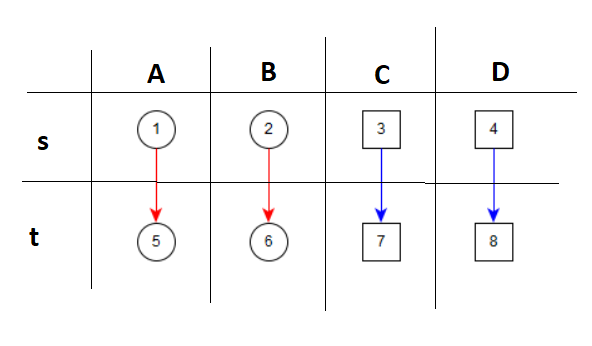
\includegraphics[scale=1]{img/suspect1.png}
\caption{\label{suspect1} $s,t$ sont deux suspect }
\end{figure}

Le lemme suivant nous permet d'affirmer qu'avoir la liste des suspects d'une DC contient toutes les violations de cette même DC \cite{main} :
\begin{mylemma}
Soit $I$ une relation sur $S$ , $\Sigma$ un ensemble de DC ,$\varphi$ une DC de $\Sigma$ et $\mathbb{C}$ une approximation de la couverture de poids minimum pour un graphe de conflit $G$ correspondant à  $\Sigma,I$ nous avons toujours $viol(I,\varphi) \subseteq susp(\mathbb{C},\varphi)$
 \end{mylemma}
 
 \begin{proof}
 Soit $I$ une instance sur $S$ , deux tuples $s,t \in I$ et $\varphi$ une DC d'un ensemble de contrainte $\Sigma$ pour $I$.\\
 Supposons que nous avons $(s,t) \in viol(I,\varphi)$ alors tous les prédicats de $\varphi$ sont vrais pour $(s,t)$ i.e $(s,t) \models \varphi$ et donc ils satisfont la condition de suspicion
 \end{proof}
 
%\begin{mydef} \cite{main}
%	L'ensemble des suspects $susp(\mathbb{C},\varphi)$ de $\varphi$ est un ensemble de tuple $(s,t)$ qui satisfont tous les prédicats dans  $\varphi$ et qui n'impliquent pas de cellules de $\mathbb{C}$.
%\end{mydef}
%
%et ils satisfont les \emph{conditions de suspicion définis comme étant}:
%
%\begin{displaymath}
%\begin{split}
%sc(s,t) &= \{I(v_1)\phi c| P: v_1 \phi c \in pred(\varphi),v_1 \in \mathbb\{C\}\}\cup \\
%	&\{I(v_1)\phi v_2| P: v_1 \phi v_2 \in pred(\varphi),v_1,v_2 \in \mathbb\{C\}\}
%\end{split}
%\end{displaymath}
%
%Toutes les violations dans la relation $I$, i.e tous les tuples $(s,t)$ avec $s,t \in I$ tel que ???, se retrouvent dans la liste de suspects, ce qui conduit à ce Lemme trivial:
%
%\begin{mylemma}
%	Pour tout $\mathbb{C}$, Nous avons toujours $viol(I,\varphi) \subseteq susp(\mathbb{C},\varphi)$
%\end{mylemma}
%
%Dès lors, si nous parvenons à obtenir tous les suspects, nous avons aussi toutes les violations.\\

\begin{myexample}

Reprenons l'exemple sur $\varphi' = \{(Revenu,>),(Taxe,>) \}$ avec comme instance $I$ le tout en relation avec le graphe de conflits à la figure \ref{grapht4}. Nous allons uniquement changer $t_4.Taxe$ comme nous l'avons fait à la table \ref{tableExample}. Donc nous prenons $\mathbb{C}$ =  $\{ t_4.Taxe \}$ and $susp(\mathbb{C},\varphi') = \{( t_4 , t_1) , 
( t_4 , t_2),
( t_4 , t_3),
( t_5 , t_4),
( t_6 , t_4),
( t_7 , t_4),
( t_8 , t_4),
( t_9 , t_4),
( t_{10} , t_4) \}$ Regardons en détails $(t_4,t_1)$ à la figure \ref{fig3}. Nous avons $t_4.Taxe \in \mathbb{C}$ représenté par un cercle et $t_1.Taxe, t_4.Revenu, t_1.Revenu \not\in \mathbb{C}$ et donc représenté par un carré. Le prédicat $t_4.Taxe > t_1.Taxe$ a une flèche rouge car il contient un cercle i.e une valeur de Taxe qui doit être changée et son opérateur $>$ est remplacé par $<$ (pour représenté la situation actuelle) et $t_4.Revenu > t1.Revenu$ ne contient pas de cercle donc sa flèche est noire i.e aucune valeur à changer. \\

Nous avons comme condition de suspicion sur $(t_4,t_1)$ : $sc(t_4,t_1,\varphi) = \{ t_4.Revenu > t_1.Revenu\}$. En se référant à la table \ref{tableMain}, nous avons $t_4.Revenu > t_1.Revenu$ ce qui implique que tous les prédicats avec une flèche bleue, c'est à dire ceux impliquant une valeur dans $\mathbb{C}$ sont satisfaits. Nous avons donc bien $(t_4,t_1)$ suspect , donc une réparation sur $t_4.Taxe$ peut introduire de nouvelles violations avec $t_1.Taxe$ , i.e $f(t_4.Taxe)$ < $t_1.Taxe$ avec $f$ fonction de réparation pour la relation I.
\end{myexample}

\begin{figure}
	\centering
	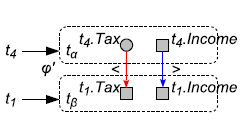
\includegraphics[scale=1]{img/fig3}
	\caption{\label{fig3}Les conditions de suspicions sont} représentées par des flèches bleues et le contexte de réparation \\
	est représenté par des flèches rouges (avec l'opérateur inverse) \\
\end{figure}

\subsubsection{Contexte de réparation}

Pour chaque couple de tuples $(s,t)\in susp(\mathbb{C},\varphi)$ nous pouvons définir un \emph{contexte de réparation} de la DC $\varphi$ qui se note $rc(s,t\varphi)$. Ce contexte de réparation nous permettra d'assurer que les réparations ne vont pas introduire de nouvelles violations. Le contexte de réparation d'une DC $\varphi$ est défini comme étant:

\begin{mydef}
Soit $I$ une relation sur $S$, soit $\varphi$ une DC sur $I$, soit $s,t \in I$, et $f$ une fonction de réparation pour I le contexte de réparation de $\varphi$ est noté $rc(s,t,\varphi)$ et vaut:

\begin{displaymath}
	\begin{split}
		rc(s,t,\varphi) = 
		&\{ t.A \overline{\theta} f(s.A) | (A,\Theta) \in pred(\varphi) , s,t \in I \}\cup\\
		&\{ f(t.A) \overline{\theta} s.A | (A,\Theta) \in pred(\varphi) , s,t \in I  \}\cup\\
		&\{ f(t.A) \overline{\theta} f(s.A) | (A,\Theta) \in pred(\varphi) , s,t \in I  \}
	\end{split}
\end{displaymath}

\end{mydef}
Si nos reprenons notre figure \ref{suspect1}  ou \ref{fig3}, les arcs rouges représentent le contexte de réparation.
 
\begin{myprop}
 Soit $I$ une relation sur $S$ et $\Sigma$ un ensemble de DC pour $I$. Toute relation $I'$ issue de la réparation de $I$ i.e $I' = f(I)$ est \emph{valide} si $I'$ satisfait tous les contextes de réparations.
\end{myprop}

\begin{myexample} (suite)
Pour le couple de suspect $(t_4,t_1) \in susp(\mathbb{C},\varphi)$ nous avons le contexte de réparation $rc(t_4,t_1,\varphi) = \{ t_4.Taxe \geq t_1.Taxe \}$ que l'on obtient en prenant l'opposé de l'opérateur du prédicat $(Taxe, <)$ (voir définition) ce qui est représenté par une flèche rouge dans la figure \ref{suspect1}. En considérant toutes les paires de tuples de $susp(\mathbb{C},\varphi)$, nous obtenons l'entièreté du contexte de réparation de $\varphi$ visible graphiquement à la figure \ref{context}. Par les contextes de réparations de $\varphi$ : $f(t_4.Taxe) > t_1.Taxe = 0$ et $f(t_4.Taxe) \leq t_5.Taxe = 0$ par transitivité , nous pouvons affirmer avec certitude que la variable fraiche $fv$ que nous avions assigné vaut $fv = 0$.
\end{myexample}

Nous avons défini le contexte de réparation pour une DC $\varphi$. Nous pouvons maintenant définir le contexte de réparation pour un ensemble $\Sigma$ de DC : 
\begin{mydef}
	$$rc(\mathbb{C},\Sigma) = \bigcup_{(s,t) \in susp(\mathbb{C},\varphi), \varphi \in  \Sigma} rc(s,t,\varphi)$$
\end{mydef}

\begin{figure}
\centering
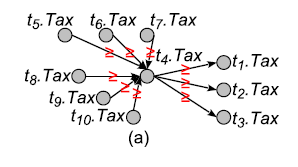
\includegraphics[scale=1]{img/context.png}
\caption{\label{context} Contexte de réparation}
\end{figure}

Nous pouvons exprimer le problème de réparation d'une relation $I$ comme étant un problème de minimisation à résoudre : \\

$\min \sum_{t. \in \mathbb{C}} dist(t.A,f(t.A))$ \\
sous la contrainte$ rc(\mathbb{C} , \Sigma)$

Il est possible d'utiliser la programmation linéaire pour résoudre ce problème d'optimisation pour les valeurs numériques et une "value frequency map" pour les chaines de caractères \cite{main}.\\

Nous pouvons décomposer $\C$ en plusieurs sous ensemble $\C_1 , \C_2,...,\C_n$ tel que $\forall s,t \in I$, il n'existe pas de $f(t.A) \overline{\Theta_A} f(s.A) \in rc(s,t,\varphi)$ pour $(s,t) \in susp(\C,\varphi)$ avec $\varphi \in \Sigma$ et $\Sigma$ un ensemble de DC pour la relation $I$ sur $S$. Nous pouvons dire que $rc(\C,\Sigma) = rc(\C_1,\Sigma) \cup ... \cup rc(\C_n,\Sigma) $ et donc nous pouvons résoudre notre problème en résolvant chaque $rc(\C_k , \Sigma)$ individuellement.

%\subsection{Algorithme de réparation de donnée}
%
%Maintenant nous pouvons décrire l'algorithme de réparation de données
%
%\IncMargin{1em}
%\begin{algorithm}
%\label{theta}
%
%	\DontPrintSemicolon
%  \caption{DATAREPAIR$(\Sigma,I,\C,\delta_{min}$}
%  \LinesNumbered
%    \SetKwInOut{Input}{Entréé}
%    \SetKwInOut{Output}{Sortie}
%
%   % \underline{$\theta$-TolerantRepair} $(\mathbb{D},\Sigma,I)$\;
%    \Input{une relation $I$ sur $S$, un ensemble de DC $\Sigma$, l'ensemble $\C$ des cellules impliquées dans la réparation, une borne $\delta_{min}$ pour le coût de réparation des données }
%    \Output{Une assignation de valeurs et de variables fraiches pour les éléments de $\C$ donnant une réparation $I'$}
%    
%    initialiser $rc(\C,\Sigma)$ et décomposer en $\C_1, ... ,\C_n$ \;
%    \Pour{chaque $\C_k$ de $\C$}{
%     \While{$\C_k \neq \emptyset$}{
%      \Si{il existe un}{}
%     
%     }
%    }
%
%
%\end{algorithm}\DecMargin{1em}

\chapter{Différence par rapport à l'article de base}

Dans ce chapitre, nous parlerons des différences entre l'article de référence sur le modèle $\theta$-tolérant et ce mémoire. Certaines notions et définitions ont été revues, et le traitement théorique a été amélioré. Certaines erreurs ont été corrigées notamment des erreurs concernant les variations de contraintes et coût de réparation de la base de données.\\

Pour la rédaction de ce mémoire, nous nous sommes inspiré de deux articles. Le premier est un article sur le modèle $\theta$-tolérant, le second est un article qui porte sur les denial constraints. Ils utilisent une approche différente et une définition différente de la notre. Dans les deux articles \cite{main,DCs} ils définissent une DC comme étant:

\begin{mydef}
	Considérons un schéma de relation $R$ avec comme attributs $att(R)$. Soit l'espace de prédicat $\mathbb{P}$ qui est un ensemble de prédicat P de la forme $v_1 \phi v_2$ ou $v_1 \phi c$ avec $v_1,v_2\ \in \ t_x.A,\ x \in \{\alpha,\beta \}$, $t_\alpha,t_\beta \in$ $R$, $A \in attr(R)$, $c$ une constante et $\phi$ $\in \{=,<,>,\leq,\geq,\neq \} $ est un opérateur. Une \emph{denial constraint} (DC)
	$$ \varphi : t_\alpha,t_\beta,... \in R,\neg(P_1 \wedge P_2 \wedge ... \wedge P_m)$$
	signifie que pour tout tuples $t_\alpha,t_\beta$ dans $R$, tous les prédicats $P_i \in pred (\varphi)$ , $i$ = 1,....,$m$, ne devraient pas être tous vrais en même temps. 
\end{mydef}

Une DC peut donc être vue comme une conjonction de prédicats et l'un de ses prédicats doit être faux afin que la DC soit vraie, i.e si pour deux tuples chaque prédicat est vrai, alors il y a au moins une donnée erronée dans l'un des deux tuples.\\

La définition bien qu'étant différente d'un point syntaxique représente toutes les deux la même chose. Cette définition-ci permet en plus de comparer un attribut à une constante. Bien qu'il puisse être intéressant d'avoir des denial contraints qui fixe un salaire minimum par exemple $t.Revenu > 10k$ ou exprime le fait qu'un revenu ou une taxe ne peut être négative $(t.Revenu >0) \wedge (t.Taxe >0)$ cela crée plusieurs problèmes.\\

\begin{figure}
	\centering
	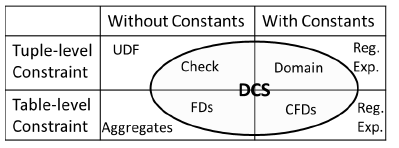
\includegraphics[scale=1]{img/quadran.png}
	\caption{La denial constraint tel que définie dans les articles }de référence peut exprimer plusieurs types
	 d'autres contraintes \cite{DCs}
\end{figure}

Dans notre définition, nous avons un nombre de prédicats maximum qui est la norme de $S$. Ici nous ne sommes pas limités et ce à cause des constantes. Et cela peut générer des problèmes lorsque l'on tente de changer une DC lors de la réparation. En effet, si notre DC est de la forme $\varphi = \neg(t.A >10)$ doit-on considérer toutes les variations possibles ($\varphi' = \neg(t.A >11)$,$\varphi'' = \neg(t.A >12)$)? Et malgré que cela puisse être un problème, ce n'est jamais abordé dans l'article \cite{main}.\\

Concernant les variations de contraintes, pour les auteurs de l'article, modifier un prédicat consiste à le supprimer puis le remplacer par un autre différent. Ce concept comporte un problème: toutes les modifications ne devraient pas être traités de la même façon. Par exemple si notre prédicat est de $(A,<)$ il devrait être moins couteux de le modifier en $(A,\leq)$ que de le modifier en $(A, \geq)$. En effet, pour modifier $\{ < \}$ en $ \leq \equiv \{<,= \}$ , il suffit d'ajouter l'opérateur $=$. Pour modifier $\{ <\}$ en $\geq \equiv \{ >,=\}$ il faut ajouter $=$ mais aussi ajouter $>$, et retirer $<$. Notre système de treillis reflète mieux le fait que la seconde modification est plus grande et donc plus couteuse.

\chapter{Implémentation}

Nous avons décidé d'implémenter l'algorithme $\theta$-tolérant en utilisant les différents concepts vus lors des chapitres précédents pour tester son efficacité. Dans ce chapitre, nous expliquerons comment nous avons implémenté les différentes notions. Nous ne donnerons pas toutes les explications du code car le code joint avec ce mémoire comporte des commentaires suffisamment explicites. Nous détaillerons les idées générales, les choix d'implémentations tels que le langage choisi, le format des bases de données, ... Nous terminerons par une discussion à propos de l'efficacité de l'algorithme, du choix de la valeur de $\theta$ , etc.

\section{Choix de langage et format de base de données}

Le langage de programmation que nous avons choisi est le Python et le développement de l'outil s'est fait avec \emph{Jupyter Notebook}, une application web et open-source qui permet de créer et partager du code , des équations, etc. Cet outil est utilisé entre autres pour la visualisation de données, le machine learning, des simulations, transformation et nettoyage de données, etc. Il supporte plus de 40 langages de programmation incluant entre autre le Python, le Scala et R.

Le langage choisi, le python a l'avantage d'être plus facilement lisible. Puisque le but de l'implémentation est de regarder si l'algorithme est performant et fonctionne bien, un code lisible est nécessaire. Le débug est plus facile que d'autres langages comme le C++ et le Java. Puisqu'une interface utilisateur graphique n'est pas nécessaire, le python se présentait comme étant une très bonne solution.

La première chose dont nous avons besoin est de bases de données. Le choix a été fait de les stocker dans des fichiers $.txt$. L'avantage de ce format est que ne nous sommes soumis à aucune contrainte particulière d'un SGBD, nous pourrons donc stocker des variables fraiches, des entiers et des chaines de caractères comme bon nous semble. Le but n'étant pas d'utiliser l'algorithme développé pour faire des réparations concrètes et réelles, nous n'avions donc aucunement besoin de choisir un autre format. Les fichiers textes doivent être formatés de la façon suivante:
\begin{itemize}


\item La première ligne contient le nom des attributs séparés chacun d'un espace.
\item La seconde ligne contient le type de variable parmi $str$ , $int$ et $float$.
\item Chaque ligne qui suit contient un tuple de la base de données. Chaque attribut est séparé avec un espace.

\end{itemize}

Parmi les bases de données , nous retrouvons bien évidement la relation de la table \ref{tableMain}.

\section{Code}

\subsection{Classe Predicate et DC}

Le premier choix fut de faire deux classes pour représenter les prédicats et les denial constraint.

La classe prédicat représente donc un prédicat comme nous l'avons défini, il y a donc un attribut et un opérateur pour ce prédicat. Parmi les opérateurs, nous ne retrouvons que les 6 opérateurs suivants : $ < , >, = , \neq , \geq$ et $\leq$ , les opérateurs $ \top$ et $\bot $ n'étant pas nécessaire. En effet, un prédicat avec l'opérateur $\top$ est toujours vrai, nous ne les écrivons même pas dans l'écriture abrégée dans les chapitres théoriques 2 et 3. L'opérateur $\bot$ étant toujours faux, aucune DC ne devrait l'avoir.

La classe DC est une collection (liste) de prédicats. Différentes fonctions permettent de modifier une DC ou de vérifier si une DC est respectée.
\chapter{Conclusion}
TODO

\bibliographystyle{plain}


\bibliography{biblio}

\newpage
\appendix
\end{document}